%  LaTeX support: latex@mdpi.com 
%  For support, please attach all files needed for compiling as well as the log file, and specify your operating system, LaTeX version, and LaTeX editor.

%=================================================================
\documentclass[algorithms,article,submit,pdftex,moreauthors]{Definitions/mdpi} 
% For posting an early version of this manuscript as a preprint, you may use "preprints" as the journal and change "submit" to "accept". The document class line would be, e.g., \documentclass[preprints,article,accept,moreauthors,pdftex]{mdpi}. This is especially recommended for submission to arXiv, where line numbers should be removed before posting. For preprints.org, the editorial staff will make this change immediately prior to posting.

%--------------------
% Class Options:
%--------------------
%----------
% journal
%----------
% Choose between the following MDPI journals:
% acoustics, actuators, addictions, admsci, adolescents, aerospace, agriculture, agriengineering, agronomy, ai, algorithms, allergies, alloys, analytica, animals, antibiotics, antibodies, antioxidants, applbiosci, appliedchem, appliedmath, applmech, applmicrobiol, applnano, applsci, aquacj, architecture, arts, asc, asi, astronomy, atmosphere, atoms, audiolres, automation, axioms, bacteria, batteries, bdcc, behavsci, beverages, biochem, bioengineering, biologics, biology, biomass, biomechanics, biomed, biomedicines, biomedinformatics, biomimetics, biomolecules, biophysica, biosensors, biotech, birds, bloods, blsf, brainsci, breath, buildings, businesses, cancers, carbon, cardiogenetics, catalysts, cells, ceramics, challenges, chemengineering, chemistry, chemosensors, chemproc, children, chips, cimb, civileng, cleantechnol, climate, clinpract, clockssleep, cmd, coasts, coatings, colloids, colorants, commodities, compounds, computation, computers, condensedmatter, conservation, constrmater, cosmetics, covid, crops, cryptography, crystals, csmf, ctn, curroncol, currophthalmol, cyber, dairy, data, dentistry, dermato, dermatopathology, designs, diabetology, diagnostics, dietetics, digital, disabilities, diseases, diversity, dna, drones, dynamics, earth, ebj, ecologies, econometrics, economies, education, ejihpe, electricity, electrochem, electronicmat, electronics, encyclopedia, endocrines, energies, eng, engproc, ent, entomology, entropy, environments, environsciproc, epidemiologia, epigenomes, est, fermentation, fibers, fintech, fire, fishes, fluids, foods, forecasting, forensicsci, forests, foundations, fractalfract, fuels, futureinternet, futureparasites, futurepharmacol, futurephys, futuretransp, galaxies, games, gases, gastroent, gastrointestdisord, gels, genealogy, genes, geographies, geohazards, geomatics, geosciences, geotechnics, geriatrics, hazardousmatters, healthcare, hearts, hemato, heritage, highthroughput, histories, horticulturae, humanities, humans, hydrobiology, hydrogen, hydrology, hygiene, idr, ijerph, ijfs, ijgi, ijms, ijns, ijtm, ijtpp, immuno, informatics, information, infrastructures, inorganics, insects, instruments, inventions, iot, j, jal, jcdd, jcm, jcp, jcs, jdb, jeta, jfb, jfmk, jimaging, jintelligence, jlpea, jmmp, jmp, jmse, jne, jnt, jof, joitmc, jor, journalmedia, jox, jpm, jrfm, jsan, jtaer, jzbg, kidney, kidneydial, knowledge, land, languages, laws, life, liquids, literature, livers, logics, logistics, lubricants, lymphatics, machines, macromol, magnetism, magnetochemistry, make, marinedrugs, materials, materproc, mathematics, mca, measurements, medicina, medicines, medsci, membranes, merits, metabolites, metals, meteorology, methane, metrology, micro, microarrays, microbiolres, micromachines, microorganisms, microplastics, minerals, mining, modelling, molbank, molecules, mps, msf, mti, muscles, nanoenergyadv, nanomanufacturing, nanomaterials, ncrna, network, neuroglia, neurolint, neurosci, nitrogen, notspecified, nri, nursrep, nutraceuticals, nutrients, obesities, oceans, ohbm, onco, oncopathology, optics, oral, organics, organoids, osteology, oxygen, parasites, parasitologia, particles, pathogens, pathophysiology, pediatrrep, pharmaceuticals, pharmaceutics, pharmacoepidemiology, pharmacy, philosophies, photochem, photonics, phycology, physchem, physics, physiologia, plants, plasma, pollutants, polymers, polysaccharides, poultry, powders, preprints, proceedings, processes, prosthesis, proteomes, psf, psych, psychiatryint, psychoactives, publications, quantumrep, quaternary, qubs, radiation, reactions, recycling, regeneration, religions, remotesensing, reports, reprodmed, resources, rheumato, risks, robotics, ruminants, safety, sci, scipharm, seeds, sensors, separations, sexes, signals, sinusitis, skins, smartcities, sna, societies, socsci, software, soilsystems, solar, solids, sports, standards, stats, stresses, surfaces, surgeries, suschem, sustainability, symmetry, synbio, systems, taxonomy, technologies, telecom, test, textiles, thalassrep, thermo, tomography, tourismhosp, toxics, toxins, transplantology, transportation, traumacare, traumas, tropicalmed, universe, urbansci, uro, vaccines, vehicles, venereology, vetsci, vibration, viruses, vision, waste, water, wem, wevj, wind, women, world, youth, zoonoticdis 

%---------
% article
%---------
% The default type of manuscript is "article", but can be replaced by: 
% abstract, addendum, article, book, bookreview, briefreport, casereport, comment, commentary, communication, conferenceproceedings, correction, conferencereport, entry, expressionofconcern, extendedabstract, datadescriptor, editorial, essay, erratum, hypothesis, interestingimage, obituary, opinion, projectreport, reply, retraction, review, perspective, protocol, shortnote, studyprotocol, systematicreview, supfile, technicalnote, viewpoint, guidelines, registeredreport, tutorial
% supfile = supplementary materials

%----------
% submit
%----------
% The class option "submit" will be changed to "accept" by the Editorial Office when the paper is accepted. This will only make changes to the frontpage (e.g., the logo of the journal will get visible), the headings, and the copyright information. Also, line numbering will be removed. Journal info and pagination for accepted papers will also be assigned by the Editorial Office.

%------------------
% moreauthors
%------------------
% If there is only one author the class option oneauthor should be used. Otherwise use the class option moreauthors.

%---------
% pdftex
%---------
% The option pdftex is for use with pdfLaTeX. If eps figures are used, remove the option pdftex and use LaTeX and dvi2pdf.

%=================================================================
% MDPI internal commands
\firstpage{1} 
\makeatletter 
\setcounter{page}{\@firstpage} 
\makeatother
\pubvolume{1}
\issuenum{1}
\articlenumber{0}
\pubyear{2022}
\copyrightyear{2022}
%\externaleditor{Academic Editor: Firstname Lastname}
\datereceived{} 
%\daterevised{} % Only for the journal Acoustics
\dateaccepted{} 
\datepublished{} 
%\datecorrected{} % Corrected papers include a "Corrected: XXX" date in the original paper.
%\dateretracted{} % Corrected papers include a "Retracted: XXX" date in the original paper.
\hreflink{https://doi.org/} % If needed use \linebreak
%\doinum{}
%------------------------------------------------------------------
% The following line should be uncommented if the LaTeX file is uploaded to arXiv.org
%\pdfoutput=1

%=================================================================
% Add packages and commands here. The following packages are loaded in our class file: fontenc, inputenc, calc, indentfirst, fancyhdr, graphicx, epstopdf, lastpage, ifthen, lineno, float, amsmath, setspace, enumitem, mathpazo, booktabs, titlesec, etoolbox, tabto, xcolor, soul, multirow, microtype, tikz, totcount, changepage, attrib, upgreek, cleveref, amsthm, hyphenat, natbib, hyperref, footmisc, url, geometry, newfloat, caption


%tikz stuff
%\usepackage{tikz}
\usetikzlibrary{arrows}
\tikzset{
	treenode/.style = {align=center, inner sep=0pt, font=\sffamily\bfseries, 
		text=black, draw=black, thick},
	node1/.style = {treenode, rectangle, rounded corners=5pt, fill=green!10, 
		minimum width=2em, minimum height=1.5em, text width=1.5em},
	dummy/.style = {treenode, rectangle, rounded corners=2.5pt, fill=green!10, 
		minimum width=1em, minimum height=0.75em},
	emp/.style = {treenode, circle, fill=white, minimum width=1.5em},
	none/.style = {treenode, rectangle, fill=black, minimum width=0.5em, 
		minimum height=0.5em}
}

% for our algorithms
\usepackage{algorithm}
\usepackage[noend]{algpseudocode}

%cref
%\usepackage[capitalise]{cleveref}

\usepackage{siunitx}

\usepackage{subcaption}
% for math enviroments

% graphics paths
%\usepackage{graphicx}
\graphicspath{{img/ex1/}{img/ex2/}{img/ex3/}{img/ex4/}{img/ex5/}{img/other/}{img/benchmark/}}

% pretty C++
\newcommand{\CC}{C\nolinebreak\hspace{-.05em}\raisebox{.4ex}{\tiny\bf ++}}

%=================================================================
%% Please use the following mathematics environments: Theorem, Lemma, Corollary, Proposition, Characterization, Property, Problem, Example, ExamplesandDefinitions, Hypothesis, Remark, Definition, Notation, Assumption
%% For proofs, please use the proof environment (the amsthm package is loaded by the MDPI class).



%=================================================================
% Full title of the paper (Capitalized)
\Title{Multiset-trie data structure}

% MDPI internal command: Title for citation in the left column
\TitleCitation{Multiset-trie data structure}

% Author Orchid ID: enter ID or remove command
%\newcommand{\orcidauthorA}{0000-0000-0000-000X} % Add \orcidA{} behind the author's name
\newcommand{\orcidauthorB}{0000-0002-3994-4805} % Add \orcidB{} behind the author's name
\newcommand{\orcidauthorC}{0000-0002-4960-8901} % Add \orcidC{} behind the author's name
\newcommand{\orcidauthorD}{0000-0001-6851-3214} % Add \orcidD{} behind the author's name

% Authors, for the paper (add full first names)
\Author{Mikita Akulich $^{1,\dagger}$, Iztok Savnik $^{1,2,\dagger}$\orcidB{}, Matjaž Krnc $^{1,2,3,\dagger}$\orcidC{}, and Riste Škrekovski $^{1,2,3,\dagger,*}$\orcidD{}}

%\longauthorlist{yes}

% MDPI internal command: Authors, for metadata in PDF
\AuthorNames{Mikita Akulich, Iztok Savnik, Matjaž Krnc, and Riste Škrekovski}

% MDPI internal command: Authors, for citation in the left column
\AuthorCitation{Akulich, M.; Savnik, I.; Krnc, K.; Škrekovski, R.}
% If this is a Chicago style journal: Lastname, Firstname, Firstname Lastname, and Firstname Lastname.

% Affiliations / Addresses (Add [1] after \address if there is only one affiliation.)
\address{%
$^{1}$ \quad 
Faculty of Mathematics, Natural Sciences and Information Technologies, \\
\hspace{4.1mm} University of Primorska, 
6000 Koper,
Slovenia;\\[1mm] %\{mikita.akulich,iztok.savnik,matjaz.krnc,riste.skrekovski\}@famnit.upr.si\\
$^{2}$ \quad 
Faculty of Information Studies, 
8000 Novo Mesto, 
Slovenia\\[1mm]
$^{3}$ \quad 
Department of Mathematics, 
Faculty of Mathematics and Physics, \\
\hspace{4.1mm} University of Ljubljana, 
1000 Ljubljana,
Slovenia\\[1mm]
}


% Contact information of the corresponding author
\corres{Correspondence: skrekovski@gmail.com %Tel.: (optional; include country code; if there are multiple corresponding authors, add author initials) +xx-xxxx-xxx-xxxx (F.L.)
%\corres{Correspondence: iztok.savnik@upr.si %Tel.: (optional; include country code; if there are multiple corresponding authors, add author initials) +xx-xxxx-xxx-xxxx (F.L.)
}


% Current address and/or shared authorship
%\firstnote{Current address: Affiliation 3.} 
\firstnote{These authors contributed equally to this work.}
% The commands \thirdnote{} till \eighthnote{} are available for further notes

%\simplesumm{} % Simple summary

%\conference{} % An extended version of a conference paper

% Abstract (Do not insert blank lines, i.e. \\) 
\abstract{
This paper proposes a new data structure \emph{multiset-trie} that is designed for storing and efficiently processing a set of multisets. Moreover, multiset-trie can operate on a set of sets without efficiency loss.
%
The multiset-trie is a search tree with properties similar to those of a trie. It implements all standard search tree operations together with the multiset containment operations for searching sub-multisets and super-multisets. Suppose we have a set of multisets $S$ and a multiset $X$. The multiset containment operations retrieve multisets from $S$ that are either sub-multisets or super-multisets of $X$. \\
%
We present the mathematical analysis of a multiset-trie that gives the time complexity of the algorithms and the space complexity of the data structure. Further, the empirical analysis of the data structure is implemented in a series of experiments. The experiments illuminate the time complexity space of the multiset containment operations.
%Finally, the comparison of the multiset-trie with the inverted index shows that the multiset-trie outperforms the inverted index by up to 4 orders of magnitude.
%%% more rounded...!
}



% Keywords
\keyword{trie data structure; multiset; containment queries} 

% The fields PACS, MSC, and JEL may be left empty or commented out if not applicable
%\PACS{J0101}
%\MSC{}
%\JEL{}

%%%%%%%%%%%%%%%%%%%%%%%%%%%%%%%%%%%%%%%%%%
% Only for the journal Diversity
%\LSID{\url{http://}}

%%%%%%%%%%%%%%%%%%%%%%%%%%%%%%%%%%%%%%%%%%
% Only for the journal Applied Sciences
%\featuredapplication{Authors are encouraged to provide a concise description of the specific application or a potential application of the work. This section is not mandatory.}
%%%%%%%%%%%%%%%%%%%%%%%%%%%%%%%%%%%%%%%%%%

%%%%%%%%%%%%%%%%%%%%%%%%%%%%%%%%%%%%%%%%%%
% Only for the journal Data
%\dataset{DOI number or link to the deposited data set if the data set is published separately. If the data set shall be published as a supplement to this paper, this field will be filled by the journal editors. In this case, please submit the data set as a supplement.}
%\datasetlicense{License under which the data set is made available (CC0, CC-BY, CC-BY-SA, CC-BY-NC, etc.)}

%%%%%%%%%%%%%%%%%%%%%%%%%%%%%%%%%%%%%%%%%%
% Only for the journal Toxins
%\keycontribution{The breakthroughs or highlights of the manuscript. Authors can write one or two sentences to describe the most important part of the paper.}

%%%%%%%%%%%%%%%%%%%%%%%%%%%%%%%%%%%%%%%%%%
% Only for the journal Encyclopedia
%\encyclopediadef{For entry manuscripts only: please provide a brief overview of the entry title instead of an abstract.}

%%%%%%%%%%%%%%%%%%%%%%%%%%%%%%%%%%%%%%%%%%
% Only for the journal Advances in Respiratory Medicine
%\addhighlights{yes}
%\renewcommand{\addhighlights}{%

%\noindent This is an obligatory section in “Advances in Respiratory Medicine”, whose goal is to increase the discoverability and readability of the article via search engines and other scholars. Highlights should not be a copy of the abstract, but a simple text allowing the reader to quickly and simplified find out what the article is about and what can be cited from it. Each of these parts should be devoted up to 2~bullet points.\vspace{3pt}\\
%\textbf{What are the main findings?}
% \begin{itemize}[labelsep=2.5mm,topsep=-3pt]
% \item First bullet.
% \item Second bullet.
% \end{itemize}\vspace{3pt}
%\textbf{What is the implication of the main finding?}
% \begin{itemize}[labelsep=2.5mm,topsep=-3pt]
% \item First bullet.
% \item Second bullet.
% \end{itemize}
%}

%%%%%%%%%%%%%%%%%%%%%%%%%%%%%%%%%%%%%%%%%%
\begin{document}

%%%%%%%%%%%%%%%%%%%%%%%%%%%%%%%%%%%%%%%%%%

\section{Introduction} \label{c:introduction}
%
% general intro into problem
%
A multiset is a data structure that represents a collection of elements. It generalizes a set data structure by allowing duplicate elements in a collection. Multisets appear in a wide variety of domains and applications. The index structures for storing sets of multisets were studied in the area of object-relational database systems to efficiently store, compress and query multiset-valued attributes \cite{bouros2016set,gripon2012compressing,ross2004symmetric,steinruecken2015compressing}. Furthermore, the need to efficiently store and query the multisets appears also in the information retrieval \cite{}, the data mining \cite{}, and in the area of expert systems \cite{}. 
%
% problem

In this paper, we address the problems of storing, indexing and querying the sets of multisets. In particular, we deal with the design of an index data structure that provides an efficient implementation of the containment queries. Let $S$ be an index storing a set of multisets. For a given input multiset $m$, a \emph{containment query} searches for either sub-multisets or super-multisets of $m$ in $S$. 

Existent indexes for storing a set of multisets are rooted in the search trees. The elements of a search tree can be accessed through keys. This approach is efficient for checking the membership of individual multisets $m$ in $S$. However, it is not as efficient for operations that use containment relation between multisets. The search based on the containment relation requires access to the collections $C\subseteq\/S$ of multisets that are related to a multiset $m$ either by a sub-multiset or a super-multisets relationship.

The existing solutions to the implementation of the containment queries include the inverted file \cite{}, signature tree \cite{} or B+ tree~\cite{Helmer2003}. These solutions provide a key-value look-up for elements of a multiset implying that containment operations are still element-wise. (? Is it possible to state more precisely the drawbacks of these solutions? ?)
%

---------------------------------------------------------------------

% description of innovations
%
To improve the efficiency of containment operations, we propose a data structure \emph{multiset-trie} that is designed for storage and processing of a finite bounded set of multisets. It extends the \emph{set-trie} data structure proposed by Savnik~\cite{savnik2013index} that was designed for storage and processing of a finite bounded (?or unbounded?) set of sets. 
%
Set-trie is a trie based data structure that provides a fast search and retrieval of sets and implements set-containment operations. 
%
Multiset-trie generalizes set-trie and can work with a set of sets (as set-trie) or with 
a set of multisets providing efficient multiset-containment operations.

% intro into mstrie
The multiset-trie is an $n$-ary tree based data structure with properties similar to those of a trie. 
Multisets are associated with a collection of nodes in a tree such that every node represents an element 
of a multiset with particular multiplicity bounded by a node degree $n.$
%
Multiset-trie is a kind of search tree. Similarly to a trie, it uses common prefixes for shared data representation.
Unlike the compact prefix tree, the multiset-trie does not support path compression. However, the absence of path 
compression makes the multiset-trie a perfectly height-balanced tree. Moreover, when multiset-trie is full it forms 
a complete $n$-ary tree.
%
The multiset-trie handles multisets directly by having access to each of the element 
without the need to reconstruct them for processing, which allows fast retrieval and 
containment operations. In particular, it supports submultiset and supermultiset queries.
The operations allow to find and retrieve the closest submultisets or supermultisets 
as well as to find and retrieve all of them.

% --------------------------------------------------------------------------------------------------------------------------------------------------------------------

% key results
Empirical studies on real data show, that multiset-trie is sensitive to the context, which can 
be further used to optimize data structure for particular data. Moreover, knowing the data 
it is possible to estimate the overall performance of the multiset-trie both time and space 
related using our mathematical theory that describes multiset-trie.
%
The comparative study shows how efficient multiset-trie is by outperforming inverted file in 
both equality and containment queries by up to 4 orders of magnitude in the time consumed by 
query. 

% --------------------------------------------------------------------------------------------------------------------------------------------------------------------

% paper organization
%
In the following Section~\ref{c:description} we present the organization of 
multiset-trie data structure in detail.
%
Next, in Section~\ref{c:operations} we present operations that multiset-trie currently 
supports. This includes multiset containment and the basic search tree functions. 
The algorithms in pseudo code are presented as well. 
%
The description of multiset-trie functions and procedures is followed by the 
mathematical analysis of their complexity in Section~\ref{c:analysis}. 
The main assumption is that multisets are constructed uniformly at random 
with bounded cardinality. By using probabilistic tools we describe time complexity of 
the algorithms and space complexity of the structure.
%
Further, in Section~\ref{c:experiments} we present an empirical study of the 
multiset-trie. Synthetic and real-world data sets are used in experiments to test the performance 
of the data structure. The experiments also highlight the methods for optimizing a multiset-trie.
%
The related work is reviewed in Section~\ref{c:relwork}. 
%
Finally, we conclude with the discussion of future work in Section~\ref{c:conclusions}.
%
% section 2
\section{Multiset-trie data structure} \label{c:description}
%
Let $\Sigma$ be a set of distinct symbols that define an alphabet and let 
$\sigma$ be the cardinality of $\Sigma.$ The \emph{multiset-trie} data structure 
stores multisets that are composed of symbols from the alphabet $\Sigma.$ It 
provides the basic tree data structure operations such as insert, delete and 
search together with multiset containment and membership operations such as 
submultiset and supermultiset that will be discussed in the next section 
in greater details.

Multiset ignores the ordering of its elements by definition, which allows us to 
define a bijective mapping $\phi:\Sigma \rightarrow I,$ where $I$ is the set of 
integers $\{ 1,2,3, \ldots, \sigma \}.$ In this way, we obtain an indexing of 
elements from the alphabet $\Sigma,$ so we can work directly with integers 
rather then with specific symbols from $\Sigma.$

The multiset-trie is an $n$-ary tree based data structure with the properties of 
trie. A node in multiset-trie always has degree $n,$ i.e. $n$ children. Some of 
the children may be \emph{Null} (non-existing), but the number of \emph{Null} 
children can be at most $n-1.$ All the children of a node, including the \emph{Null} 
children, are labeled from left to right with labels $c_j,$ where $j\in \{ 0, 1, \ldots, n-1 \}.$ 
Every two child nodes $u$ and $v$ that share the same parent node have different labels.

%The multiset-trie is an $n$-ary tree based structure. A node can have a degree 
%from $1$ to $n,$ depending on the number of existing children. The edges from 
%parent node to children have labels $c_j,$ where $j\in \{ 0, 1, \ldots, n-1 \}.$ 
%The edges are labeled from left to right with the condition that there are no 
%two edges with the same label coming from a parent node. 

Nodes that have equal height in a multiset-trie form a level. The height of a 
multiset-trie is always $\sigma+1$ if at least one multiset is in structure. 
The height of the root node (the first level) is defined to be 1.
%
Levels in multiset-trie are enumerated by their height, i.e. a level $L_i$ has 
height $i.$ The connection between level height in a multiset-trie and symbols 
from alphabet $\Sigma$ is defined as follows. A level $L_i,$ where 
$i\in\{ 1,2,\ldots, \sigma \}$ represents a symbol $s\in\Sigma,$ such that 
$\phi^{-1}(i) = s.$ The last level $L_{\sigma+1}$ does not represent any symbol 
and is named \emph{leaf level} ($LL$ for short).

Since every level, except $LL$ represents a symbol from $\Sigma,$ we can define 
a transition between nodes that are located at different levels in a multiset-trie. 
%
Consider two nodes $u,v$ in a multiset-trie at levels $L_i, L_{i+1}$ respectively, 
where $i\in\{1,2,\ldots,\sigma\}.$ Let a node $u$ be a parent node of a node $v$ 
and consequently a node $v$ be a child node of a node $u.$ Suppose that a child 
node $v$ is not \emph{Null} and has a label $c_j,$ where $j\in\{ 0,1,\ldots, n-1 \}.$ 
%
Then the \emph{path} $u\rightarrow v$ represents a symbol $s\in\Sigma$ with 
multiplicity $j,$ such that $\phi^{-1}(i) = s.$ 
%
Such a transition $u\rightarrow v$ is called a \emph{path of length} $1$ and is 
allowed if and only if a node $v$ is not \emph{Null} and $u$ is a parent node of 
a node $v.$ If a node $v$ has label $c_0,$ then the path $u\rightarrow v$ 
represents a symbol with the multiplicity $0$ respectively i.e. an empty symbol.

We define a \emph{complete path} to be the path of length $\sigma$ in a 
multiset-trie with the end points at root node (the 1st level) and $LL$. Thus, 
a multiset $m$ is inserted into a multiset-trie if and only if there exists a 
complete path in a multiset-trie that corresponds to $m.$
%
Note that every complete path in a multiset-trie is unique. Therefore, the multisets 
that share a common prefix in a multiset-trie can have a common path of length at 
most $\sigma-1.$ The complete path that passes through nodes labeled by $c_0$ 
on all levels represents an empty multiset or an empty set.
%
Thus, any multiset $m$ that is composed of symbols from $\Sigma$ with maximum 
multiplicity not greater than $n-1$ can be represented by a complete path in a multiset-trie.

Let us have an example of a multiset-trie data structure. Let $\sigma = 2$ and 
$\Sigma = I = \{ 1,2 \}$ respectively, so the mapping $\phi$ is an identity mapping. 
Fix the degree of a node $n=3,$ so the maximal multiplicity of an element in 
a multiset is $n-1=2.$ The figure~\ref{fig:sketch} presents the multiset-trie that 
contains multisets $\emptyset, \{ 1,1,2 \},$ $\{ 1,2,2 \},$ $\{ 2 \},$ $\{ 1,2 \},$ $\{ 2,2 \}.$ 
The \emph{Null} children are omitted on the figure.

\begin{figure}[h!]
\centering
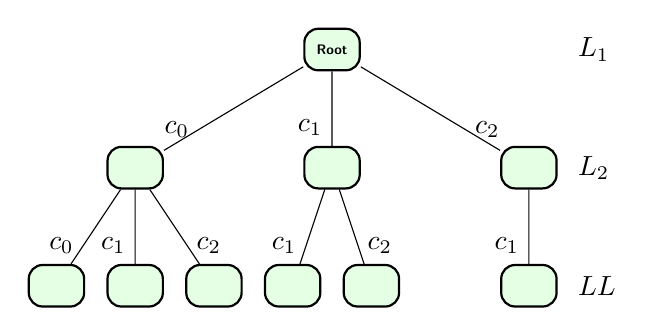
\begin{tikzpicture}[>=stealth',
level 1/.style={sibling distance = 2.5cm},
level 2/.style={sibling distance = 1cm},
level distance = 1.5cm]
\node (R) [node1] {\tiny Root}
	child { node [node1] {} 
		child { node [node1] {} edge from parent node [near end, left] {$c_0$}}
		child { node [node1] {} edge from parent node [near end, left] {$c_1$}}
		child { node [node1] {} edge from parent node [near end, right] {$c_2$}}
		edge from parent node [near end, left] {$c_0$}	
	}
	child { node [node1] {}
		child { node [node1] {} edge from parent node [near end, left] {$c_1$}}
		child { node [node1] {} edge from parent node [near end, right] {$c_2$}}
		edge from parent node [near end, left] {$c_1$}
	}
	child { node [node1] {} 
		child { node [node1] {} edge from parent node [near end, left] {$c_1$}}
		edge from parent node [near end, right] {$c_2$} 
};	
%----------------- Level labels --------------	
	\begin{scope}[every node/.style={right}]
		\path (R 				-| R-3-1) ++(5mm,0) node {$L_1$};
		\path (R-3 			-| R-3-1) ++(5mm,0) node {$L_2$};
		\path (R-3-1		-| R-3-1) ++(5mm,0) node {$LL$};
	\end{scope}			
\end{tikzpicture}
\caption{Example of multiset-trie structure.}
\label{fig:sketch}
\end{figure}

Let a pair $(L_i, c_j)$ represents a node with label $c_j$ at a level $L_i.$ 
The pair $(L_1,c_j)$ is equivalent to $(L_1,root),$ since the first level has 
the root node only. According to the figure~\ref{fig:sketch} we can extract 
inserted multisets as follows:

\begin{eqnarray*}
(L_1,root) \rightarrow (L_2,c_0) \rightarrow (LL,c_0) & = & \{ 1^0, 2^0 \} = \emptyset \\
(L_1,root) \rightarrow (L_2,c_0) \rightarrow (LL,c_1) & = & \{ 1^0, 2^1 \} = \{ 2 \} \\
(L_1,root) \rightarrow (L_2,c_0) \rightarrow (LL,c_2) & = & \{ 1^0, 2^2 \} = \{ 2,2 \} \\
(L_1,root) \rightarrow (L_2,c_1) \rightarrow (LL,c_1) & = & \{ 1^1, 2^1 \} = \{ 1,2 \} \\
(L_1,root) \rightarrow (L_2,c_1) \rightarrow (LL,c_2) & = & \{ 1^1, 2^2 \} = \{ 1,2,2 \} \\
(L_1,root) \rightarrow (L_2,c_2) \rightarrow (LL,c_1) & = & \{ 1^2, 2^1 \} = \{ 1,1,2 \} 
\end{eqnarray*}
where $e^k$ represents an element $e$ with multiplicity $k.$
% section 3
\section{Multiset-trie operations} \label{c:operations}

%
Let $\mathcal{M}$ be a multiset-trie and let $M$ be a set of multisets that are 
inserted into the multiset-trie $\mathcal{M}.$ We define a type \emph{Multiset} in 
order to use it as a representation of a multiset. The type \emph{Multiset} is 
an array $m$ of constant length $\sigma,$ where $i$-th cell represents the element 
$\phi^{-1}(i)$ from $\Sigma$ with multiplicity $m[i].$ From now on, we 
agree that the first cell of an array has index 1. Let us have an example of a 
\emph{Multiset} instance with $\sigma = 2:$
%
\begin{center}
\begin{tabular}{ccc}
Multiset & & Instance of type Multiset \\
$\{ 1,1,2 \}$ & $\cong $ & 
\begin{tabular}{|c|c|}
\hline 
2 & 1 \\
\hline 
\multicolumn{1}{c}{\tiny 1} & \multicolumn{1}{c}{\tiny 2} \\
\end{tabular}
\end{tabular}
\end{center}
%
The operations supported by the multiset-trie data structure are as
follows. 
%
\begin{enumerate}
\item \textsc{insert}($\mathcal{M}$, $m$): inserts a multiset $m$ into 
$\mathcal{M}$ if $m\not\in M;$
%
\item \textsc{search}($\mathcal{M}$, $m$): returns true if a multiset $m\in M$ 
for a given $\mathcal{M},$ and returns false otherwise;
%
\item \textsc{delete}($\mathcal{M}$, $m$): returns true if a multiset $m$ was 
successfully deleted from $\mathcal{M},$ and returns false otherwise (in case 
$m\not\in M$);
%
\item \textsc{submsetExistence}($\mathcal{M}$, $m$, $dev$): returns true if 
there exists a $x\in M$ for a given $\mathcal{M}$ such that $x\subseteq m$ 
and $| x[i] - m[i] |\leq dev$ for $1\leq i\leq \sigma$, and returns false otherwise; 
%
\item \textsc{supermsetExistence}($\mathcal{M}$, $m$, $dev$): returns true if 
there exists a $x\in M$ for a given $\mathcal{M}$ such that $x\supseteq m$ 
and $| x[i] - m[i] |\leq dev$ for $1\leq i\leq \sigma$, and returns false otherwise; 
%
\item \textsc{getAllSubmsets}($\mathcal{M}$, $m$, $dev$): returns the set of multisets 
$\{ x \in M : x\subseteq m \wedge |x[i]-m[i]|\leq dev \}$ for a given 
$\mathcal{M},$ where $1\leq i\leq \sigma;$
%
\item \textsc{getAllSupermsets}($\mathcal{M}$, $m$, $dev$): returns the set of multisets 
$\{ x\in M : x\supseteq m \wedge |x[i]-m[i]|\leq dev \}$ for a given $\mathcal{M},$
where $1\leq i\leq \sigma.$
%
\end{enumerate}

The parameter $dev$ is used to specify the maximal deviation in the multiplicity
of multiset containment operations. It is utilized to limit the search in multiset
containment queries to the sub-multisets and super-multisets that are
the closest to the input multiset $m$. In addition, we use $dev$ for
the implementation of multiset similarity search that, given $m$, retrieves
from $\mathcal{M}$ all sub-multisets or super-multisets that are similar to $m$
with respect to the deviation $dev$.

In the following subsections, we will present each operation of the multiset-trie 
data structure separately. 

Firstly we would like to describe some notations that will be used. The 
multiset-trie data structure is a recursive data structure. Hence, any subtree 
of a multiset-trie $\mathcal{M}$ is again a multiset-trie. This fact allows 
us to use the root node of a multiset-trie as its representative. Thus, the notation 
$\mathcal{M}$ will be used instead of $\mathcal{M}.root$ to refer to the root 
node of $\mathcal{M}.$ Non-existing or \emph{Null} nodes in multiset-trie will 
be marked as \emph{Null} and existing nodes at the level $LL$ will be marked 
as \emph{accepting} nodes. The array slicing operation will be used as follows. 
For a given array $a,$ $a[i:]$ represents the array obtained from $a$ by taking 
only the cells from index $i$ until the last cell. 


\subsection{Insert} \label{s:insert}
The procedure \textsc{insert}($\mathcal{M}$, $m$) inserts a new instance $m$ of 
type Multiset into multiset-trie $\mathcal{M}$. If the complete path already 
exists, then the procedure leaves the structure unchanged. Otherwise, it extends 
partially existing or creates a new complete path. The procedure does not return 
any result. The pseudocode for procedure \textsc{insert} is presented in 
Algorithm~\ref{alg:insert}.


\begin{algorithm}[h!]
\caption{Procedure \textsc{insert}}
\label{alg:insert}
\begin{algorithmic}[1]
\Procedure{\textsc{insert}}{$\mathcal{M}$, $m$}
\State $currentNode \gets \mathcal{M}$
\For{$i=1$ to $\sigma$}
\If {child $c_{m[i]}$ of $currentNode$ is \emph{Null}}
\State create new child $c_{m[i]}$ of $currentNode$
\EndIf
\State $currentNode \gets c_{m[i]}$
\EndFor
\State mark $currentNode$ as \emph{accepting}
\EndProcedure
\end{algorithmic}
\end{algorithm}

\subsection{Search}\label{s:search}
The function \textsc{search}($\mathcal{M}$, $m$) checks if the complete path corresponding to 
a given multiset $m$ exists in the structure $\mathcal{M}.$ The function returns 
true if the multiset $m$ exists in $\mathcal{M}$, and returns false otherwise. The 
function \textsc{search} is presented in Algorithm~\ref{alg:search}.

\begin{algorithm}[h!]
\caption{Function \textsc{search}}
\label{alg:search}
\begin{algorithmic}[1]
\Function{\textsc{search}}{$\mathcal{M}$, $m$}
\State $currentNode \gets \mathcal{M}$
\For{$i=1$ to $\sigma$}
\If {child $c_{m[i]}$ of $currentNode$ is \emph{Null}}
\State \Return False
\EndIf
\State $currentNode \gets c_{m[i]}$
\EndFor
\State \Return True
\EndFunction
\end{algorithmic}
\end{algorithm}

\subsection{Delete} \label{s:delete}
Function \textsc{delete}($\mathcal{M},$ $m$) searches for the complete path 
that corresponds to $m$ in order to remove it. If the path can not be found, the 
function immediately returns false. During the search, the function keeps track of the 
number of children for every node. It marks the nodes that have more than one child 
as \emph{parent nodes} and remembers the label of the child, which is a potential node 
where the sub-tree will be cut to remove the multiset. The parent node is needed to 
perform a removal because the multiset-trie is an explicit data structure. When the search 
is completed, the function removes the sub-tree of the last found parent node and 
returns true. In such a way, after deletion, all the prefixes for other multisets are 
preserved in $\mathcal{M}$ and $m$ is removed. The function \textsc{delete} is 
presented in Algorithm~\ref{alg:delete}.


\begin{algorithm}[h!]
\caption{Function \textsc{delete}}
\label{alg:delete}
\begin{algorithmic}[1]
\Function{\textsc{delete}}{$\mathcal{M},$ $m$}
\State $currentNode \gets \mathcal{M}$
\State $parent \gets currentNode$ 
\State $position \gets 1$
\For {$i=1$ to $\sigma$}
\If {child $c_{m[i]}$ of $currentNode$ is \emph{Null}}
\State \Return False
\EndIf
\State $numChildren \gets 0$
\For {$j=0$ to $n-1$}
\If {child $c_j$ of $currentNode$ is not \emph{Null}}
\State $numChildren\gets numChildren+1$
\EndIf
\EndFor
\If {$numChildren$ is not $1$}
\State $parent\gets currentNode$
\State $position \gets i$
\EndIf
\State $currentNode \gets c_{m[i]}$
\EndFor
\State child $c_{m[position]}$ of $parent\gets$ \emph{Null}
\State \Return True
\EndFunction
\end{algorithmic}
\end{algorithm}

\subsection{Sub-multiset and super-multiset existence}
\label{s:subexists} \label{s:superexists}
The functions \textsc{submsetExistence} and \textsc{supermsetExistence} are
symmetrical in the following sense. Let a multiset $m$ represent the borderline
in $\mathcal{M}$ defined by a path from the root to a leaf by following
the elements from $m$. The operation \textsc{submsetExistence} searches
the left part of $\mathcal{M}$ and the operation \textsc{supermsetExistence}
the right part of $\mathcal{M}$. 

The function \textsc{submsetExistence}($\mathcal{M},m,dev$) checks if there exists 
a multiset $x$ in $\mathcal{M},$ that satisfies the condition $x\subseteq m$ and 
$| x[i] - m[i] | \leq dev,$ where $1\leq i \leq \sigma.$ 
The function starts with searching for an exact match $x=m$ in $\mathcal{M},$ 
since $m\subseteq m$ by definition of sub-multiset inclusion. If an exact match is 
not found in $\mathcal{M},$ the function uses multiset-trie to find the closest 
(the largest) sub-multiset of $m$ in $\mathcal{M}$ by decreasing the multiplicity of 
elements in $m.$ The parameter $dev$ is used to limit a maximal deviation of 
multiplicity for a particular element in $x$ with respect to $m.$ 
At every level, the function tries to proceed with the largest possible multiplicity of 
an element that is provided by $m.$ However, when the function reaches some level 
where it meets a \emph{Null} node and can not go further using the path provided by 
$m,$ it decreases the multiplicity of an element 
that corresponds to a current level with respect to the specified maximal deviation. 
Thus, the function can decrease the multiplicity of an element or eventually skip it in 
order to find the closest $x\subseteq m.$ The function \textsc{submsetExistence} 
is presented in Algorithm~\ref{alg:subexists}.

\begin{algorithm}[h!]
\caption{Function \textsc{submsetExistence}}
\label{alg:subexists}
\begin{algorithmic}[1]
\Function{\textsc{submsetExistence}}{$\mathcal{M}, m, dev$}
\State $currentNode \gets \mathcal{M}$
\If {$currentNode$ is \emph{accepting}}
\State \Return True
\EndIf
\For {$i=m[1]$ down to max($0, m[1]-dev$)}
\If {child $c_i$ of $currentNode$ is not \emph{Null}}
\If {\textsc{submsetExistence}($c_i,m[2:], dev$)}
\State \Return True
\EndIf
\EndIf
\EndFor
\State \Return False
\EndFunction
\end{algorithmic}
\end{algorithm}

%\subsection{Super-multiset existence} \label{s:superexists}
The function \textsc{supermsetExistence}($\mathcal{M},m,dev$) checks if there 
exists super-multiset $x$ of a given multiset $m$ in $\mathcal{M},$ such that 
condition $| x[i] - m[i] |\leq dev$ is satisfied, where $1\leq i \leq \sigma.$
Symmetrically to the function \textsc{submsetExistence}, the function
\textsc{supermsetExistence} searches first for an exact match $x=m$ in
$\mathcal{M}.$ If such $x$ does not exist in $\mathcal{M},$ then
the function searches on the right side of the borderline (an exact match)
defined by $m$. Since we would like to find the closest (the smallest)
super-multiset we increase the multiplicity of elements in $m$ at every
level of $\mathcal(M)$ starting with the multiplicities of $m.$
The function \textsc{supermsetExistence} is presented in
Algorithm~\ref{alg:superxists}.


\begin{algorithm}[h!]
\caption{Function \textsc{supermsetExistence}}
\label{alg:superxists}
\begin{algorithmic}[1]
\Function{\textsc{supermsetExistence}}{$\mathcal{M},m,dev$}
\State $currentNode \gets \mathcal{M}$
\If {$currentNode$ is \emph{accepting} }
\State \Return True
\EndIf
\For {$i=m[1]$ to min($n-1, m[1] + dev$)}
\If {child $c_i$ of $currentNode$ is not \emph{Null}}
\If {\textsc{supermsetExistence}($c_i,$ $m[2:], dev$)}
\State \Return True
\EndIf
\EndIf
\EndFor
\State \Return False
\EndFunction
\end{algorithmic}
\end{algorithm}


\subsection{Get all sub-multisets and get all super-multisets} \label{s:getall}
The algorithms for functions \textsc{getAllSubmsets} and 
\textsc{getAllSupermsets} are based entirely on algorithms for 
\textsc{submsetExistence} and \textsc{supermsetExistence} functions that do not 
terminate on the first existing sub/super-multiset, but store the results and 
continue the procedure until all existing sub/super-multisets in $\mathcal{M}$ are 
found and stored. The functions \textsc{getAllSubmsets} and \textsc{getAllSupermsets} 
are presented in Algorithm~\ref{alg:getallsub} and Algorithm~\ref{alg:getallsup} respectively.

In order to record a multiset during multiset-trie traversal, we use the variable $x$ in the algorithms.
It is an empty array of size $\sigma$ where we store multiplicities of elements at 
each level as we traverse the tree. The variable $result$ is used as a container for storing 
sub-multisets of $m$ found during traversal. Both variables $x$ and $result$ are presented 
as global, however, they could be passed to the recursive function as parameters.

\begin{algorithm}[h!]
\caption{Function \textsc{getAllSubmsets}}
\label{alg:getallsub}
\begin{algorithmic}[1]
\State $result \gets$ empty container
\State $x \gets$ empty array of size $\sigma$
\Function{\textsc{getAllSubmsets}}{$\mathcal{M}, m, dev$}
\State $currentNode \gets \mathcal{M}$
\If {$currentNode$ is \emph{accepting}}
\State add copy of $x$ to $result$ 
\EndIf
\For {$i=m[1]$ down to max($0, m[1]-dev$)}
\If {child $c_i$ of $currentNode$ is not \emph{Null}}
\State $x[1]\gets i$
\State \textsc{getAllSubmsets}($c_i,m[2:], dev$)
\EndIf
\EndFor
\EndFunction
\end{algorithmic}
\end{algorithm}


\begin{algorithm}[h!]
\caption{Function \textsc{getAllSupermsets}}
\label{alg:getallsup}
\begin{algorithmic}[1]
\State $result \gets$ empty container
\State $x \gets$ empty array of size $\sigma$
\Function{\textsc{getAllSupermsets}}{$\mathcal{M},m,dev$}
\State $currentNode \gets \mathcal{M}$
\If {$currentNode$ is \emph{accepting} }
\State add copy of $x$ to $result$ 
\EndIf
\For {$i=m[1]$ to min($n-1, m[1] + dev$)}
\If {child $c_i$ of $currentNode$ is not \emph{Null}}
\State $x[1]\gets i$
\textsc{getAllSupermsets}($c_i,$ $m[2:], dev$)
\EndIf
\EndFor
\EndFunction
\end{algorithmic}
\end{algorithm}
% section 4
\section{Mathematical analysis of the structure} \label{c:analysis}
%
In this chapter, we present theoretical results of time and space complexity of
the multiset-trie data structure. In the following Section~\ref{s:timecomplexity} 
we discuss the running time complexity of the presented algorithms. First, in 
Section~\ref{ss:mathmodel}, we present the mathematical model that we use 
to describe the distribution of multisets in the multiset-trie and input data. 
Using a probabilistic approach and tools from a Galton-Watson process, we 
measure the expected cardinality of the multiset-trie in Theorem~\ref{thm:exp_nodes}. 
Further, we derive the expected cardinality of the searched subtree of the 
multiset-trie parametrized by an input multiset in Corollary~\ref{cor:exp_nodes_param}.

In Section~\ref{ss:getall} we discuss the running time complexity of the functions 
\textsc{getAllSubmsets} and \textsc{getAllSupermsets}. We observe that the 
complexity of functions is exponential. Moreover, the worst-case running time 
complexity is the same for both functions, and its upper bound is the cardinality of 
the multiset-trie.

The remaining "existence" functions are discussed in the Section~\ref{ss:exists}. 
We observe that out of the scope of our mathematical model, unlike in functions 
\textsc{getAllSubmsets} and \textsc{getAllSupermsets} the mapping $\phi$ has an 
impact on performance of the functions \textsc{submsetExistence} and 
\textsc{supermsetExistence}. In particular, the frequency analysis of the symbols 
from $\Sigma$ in input data determines such a $\phi$ that gives a boost in performance. 

We find that the performance of the functions \textsc{submsetExistence} and 
\textsc{supermsetExistence} in the worst-case scenario is also exponential and 
does not depend on the outcome of the functions. We give a quite precise upper 
bound for the worst-case running time complexity, which appears to be the same 
for both functions. However, it must be stressed that for the positive outcome, an 
exponential behavior holds only on specific cases, such as the presence of the empty set 
in the multiset-trie. 

Finalizing the mathematical analysis, we present the study of space complexity 
of the multiset-trie in Section~\ref{s:spacecomplexity}. We show that the space 
used for the storage is asymptotically equal to the size of the input data. 

\subsection{Time complexity of the algorithms}\label{s:timecomplexity}
The performance of the functions will be measured by the number of 
visited nodes in a multiset-trie during the execution of a particular query by the 
functions \textsc{search}, \textsc{delete}, \textsc{submsetExistence}, 
\textsc{supermsetExistence}, \textsc{getAllSubmsets}, \textsc{getAllSupermsets} 
and the procedure \textsc{insert}.
%

By the design of the multiset-trie, it is easy to see that the functions \textsc{search},
\textsc{delete} and the procedure \textsc{insert} have complexity of $O(\sigma).$
Because $\sigma$ is defined when the structure is initialized and does not depend
on the user input afterwards, the asymptotic complexity of the functions \textsc{search}, 
\textsc{delete} and the procedure \textsc{insert} is $O(1).$ Nonetheless, in the general 
case, the complexity is $O(\sigma).$

In what follows, we focus on the analysis of the more involved functions:
\textsc{submsetExistence}, \textsc{supermsetExistence}, \textsc{getAllSubmsets}
and \textsc{getAllSupermsets}.

\subsubsection{Mathematical model} \label{ss:mathmodel}
We start with the basics of our mathematical model. Let $\Sigma$ be an alphabet of
cardinality $\sigma,$ such that $\Sigma = \{ 1,2, \ldots, \sigma \}.$ Define $N$
to be the set of all possible multisets that can be inserted in a
multiset-trie. Let $n$ be the maximal degree of a node in a multiset-trie.
Then the maximal multiplicity of an element in a multiset is equal to $n-1.$
Thus, the number of multisets in a complete multiset-trie is $ |N| = n^{\sigma}.$
%
Let $M$ be a collection of multisets inserted into multiset-trie $\mathcal{M}.$
All the multisets in $M$ are constructed from the alphabet $\Sigma$ according
to the parameters $\sigma$ and $n$. Hence, any multiset $m\in M,$ 
has at most $\sigma$ distinct elements that are members of $\Sigma$ and 
every distinct element in $m$ has multiplicity strictly less than $n.$
%
Because a multiset does not distinguish different orderings, it is assumed, for
simplicity, that all elements are ordered in ascending order. A multiset $m$ is
represented as $\{1^{k_1},2^{k_2},\ldots, \sigma^{k_\sigma}\},$ where $e^{k_e}$
represents an element $e\in\Sigma$ with multiplicity $k_e.$
%

Denote the nodes of multiset-trie on all levels but on $\sigma + 1$ as \emph{internal}
and nodes on leaf level as \emph{leaf} nodes.
%
Observe that every internal non-root node has a degree at least~1. Indeed an
insertion of a multiset requires construction of a path of length~$\sigma + 1,$
meaning that if an internal node exists in a multiset-trie, it must have a degree
at least~1. It also follows that the height of a multiset-trie is always~$\sigma +1$
as soon as at least one multiset is inserted into the data structure.

Our model assumes that all the inserted multisets are chosen with the same probability,
meaning that for some $p\in (0,1)$, the following holds:
\[
P(m\in M) = p, \quad \forall~m\in N.
\]
%
Let $\xi_1, \xi_2, \ldots, \xi_{\sigma+1}$ be random variables such that $\xi_i$
represents the number of nodes in a multiset-trie on $i$-th level. For every node $j$ 
on $i$-th level we assign a random variable $\xi_{ij}$ to be the number of its children, 
such that $j\in[1,\xi_i].$ Then for every $i\in[1,\sigma]$ the following holds:
%
\begin{equation}\label{eq:sum_recursive}
\xi_{i+1} = \sum_{j=1}^{\xi_i} \xi_{ij},
\end{equation}
%
where $\xi_1 = 1.$
%
It is easy to see that the variable $\xi_{i+1}$ can have values in the interval
$[\xi_i,n^{i}]$ and the value of the variable $\xi_{ij}$ is within the interval $[1,n].$
Without conditioning on the existence of any node in multiset-trie, 
it is easy to describe the probability of the existence of any individual node.

\begin{Lemma}\label{l:prob-node-existence}
Any potential node on a fixed level $i,$ where $i\in \{ 1,2,\ldots, \sigma +1 \}$ exists, %independently of others,
with probability
\begin{equation}
p_i=1-(1-p)^{n^{\sigma + 1 -i}}.
\end{equation}
\end{Lemma}
\begin{proof}
Let $v$ be an arbitrary node in a multiset-trie on an arbitrary level $i.$ Consider
the subtree with the root $v$ and call it $v$-subtree. Since the height of the
multiset-trie is $\sigma + 1$ we can calculate the height of the $v$-subtree.
Taking into account that the root node has height 1, the height of the $v$-subtree is
%
\[
h_v = \sigma + 1 - i.
\]
%
A node in a multiset-trie exists if at least one node exists on the leaf level of its
subtree, i.e. a node on the level $\sigma + 1$ that belongs to $v$-subtree. The possible
number of nodes on the leaf level of $v$-subtree can be easily calculated knowing its height.
It is equal to
%
\[
n^{\sigma + 1 - i}.
\]
%
A node at level $\sigma+1$ exists with probability $p,$ where $p = P(m\in M).$
Thus, the probability that there are no nodes on leaf level in $v$-subtree is
%
\[
(1-p)^{n^{\sigma +1 - i}}.
\]
%
The claim follows by taking the complement probability of the above result. 

%
\end{proof}

However, in order to determine the distribution of $\xi_{ij}$, one needs a lemma of a different kind.

\begin{Lemma}\label{l:prob-children}
Suppose that a node $v$ exists at level $1\leq i\leq\sigma$.
Then the number of its children $\xi_{iv}$ is modeled by a zero-truncated binomially
distributed random variable on parameters $n$ and $p_{i+1}$. In particular,
the probability of node $v$ having $k$ children equals to
\begin{equation}\label{eq:pdf}
P(\xi_{iv} = k) = \frac{\binom{n}{k} (1-p_{i+1})^{n-k}}{1-(1-p_{i+1})^n}
\end{equation}
and the corresponding probability generating function equals to
\begin{equation}\label{eq:generating_func}
G_i(z) = \frac{(1+p_{i+1}(z-1))^n - (1-p_{i+1})^n}{1-(1-p_{i+1})^n}.
\end{equation}
\end{Lemma}
\begin{proof}
In order to prove the lemma, we have to show that
$\xi_{iv}\sim\mathcal{B}_0(n, p_{i+1}).$
Consider an arbitrary node $v$ on level $1\leq i\leq\sigma.$ According to the
definition of the multiset-trie, a node exists at level $i$ if and only if
it has at least one child. Note that this is not true for the nodes on the leaf
level $\sigma + 1.$ Implies, a node on level $i$ can have
$k\in\{ 1,2,\ldots, n\}$ children. Let $X_0, X_1, \ldots, X_{n-1}$ be random
variables, they are defined as follows:
\[
X_k = \begin{cases}
0 & \textrm{child $k$ of node $v$ does not exist} \\
1 & \textrm{child $k$ of node $v$ exists} \\
\end{cases}
\]
As it was shown in previous Lemma~\ref{l:prob-children}, the distribution of 
$X_k$ is $X_k\sim Bernoulli(p_{i+1}).$ Since our model assumes that all the 
multisets in $M$ are chosen uniformly at random, the variables 
$X_k,X_l$ are independent for $k\neq l.$ But in our case the node $v$ can not 
have 0 children, so the sum $\sum_{k=1}^n X_k$ has a zero-truncated binomial 
distribution:
%
\[
\sum_{k=1}^n X_k \sim\mathcal{B}_0(n,p_{i+1})
\]
%
which completes the proof.

\end{proof}
%
Knowing the probability density and probability generating functions of $\xi_{ij}$ 
from Lemma~\ref{l:prob-children}, we can now estimate the number of nodes in 
a randomly generated multiset-trie as follows:
%
\begin{equation}\label{eq:num_nodes}
\mathbb{E}( | \mathcal{M} | ) = \mathbb{E}\left[ \sum_{i=1}^{\sigma+1} \xi_i \right].
\end{equation}
%

%Note that in a real world models multisets in $M$ are not chosen with the same 
%probability. Specifically, in some cases, the probability $P(m\in M)$ varies 
%dramatically and can be even equal to $0.$ For example, if words are mapped 
%to multisets, then the sample space $N$ contains very large multisets. However, 
%most of them will have probability $P(m\in M)=0,$ because a word that would correspond 
%to such a multiset simply does not exist. So, we can safely conclude that multiset-trie 
%is an input sensitive data structure, because the size of multiset-trie $|\mathcal{M}|$ 
%depends on the probability distribution function $P(m\in M).$
%

In order to evaluate~(\ref{eq:num_nodes}) we will use some of the tools from 
a Galton-Watson process, see Gardiner~\cite{gardiner1985stochastic} for 
an introduction.
Using the equations~(\ref{eq:sum_recursive}) and~(\ref{eq:generating_func}) we can 
derive the probability generating function for the random variable $\xi_{i+1}$ as 
\begin{equation}\label{eq:g_rec}
G_{\xi_{i+1}}(z) = G_{\xi_i}(G_i(z)).
\end{equation}
Since there is always precisely one node at the root level, we have $P(\xi_1 = 1) = 1.$ 
Hence, the probability generating function for the random variable $\xi_1$ is 
\begin{equation}\label{eq:g_xi_one}
G_{\xi_1}(z) = z^1 = z
\end{equation}
which is the initial condition for the recursive equation~(\ref{eq:g_rec}).

\begin{Proposition}\label{prop:exp_rec}
The expectation of the random variable $\xi_{i+1}$ can be expressed 
as follows.
\[
\mathbb{E}(\xi_{i+1}) = \mathbb{E}(\xi_i)\mathbb{E}(\mathcal{B}_0(n,p_{i+1}))
\]
for $1\leq i\leq\sigma.$
\end{Proposition}
\begin{proof}
Using the following property of probability generating function
\begin{equation}\label{eq:prop_exp-pgf}
G_X'(1^-) = \mathbb{E}(X)
\end{equation}
the expectation for the random variable $\xi_{i+1}$ can be derived in terms of 
the equation~(\ref{eq:g_rec}).
\begin{eqnarray}\label{eq:exp}
\mathbb{E}(\xi_{i+1}) &=& G_{\xi_{i+1}}'(1^-) \nonumber \\
&=& G_{\xi_i}'(G_i(1^-))G_i'(1^-).
\end{eqnarray}
According to~(\ref{eq:pdf}) and~(\ref{eq:generating_func}) the value of $G_i(z)$ at 
$1$ is $1$ and the value of its derivative at $1$ is $\mathbb{E}(\mathcal{B}_0(n,p_{i+1})).$ 
Substituting the values of $G_i(1^-)$ and $G_i'(1^-),$ and applying the 
property~(\ref{eq:prop_exp-pgf}) we complete the proof.

\end{proof}
%
From the Proposition~\ref{prop:exp_rec} above and Lemma~\ref{l:prob-children} we 
can conclude that 
\begin{eqnarray}
\mathbb{E}(\xi_{i}) &=& \mathbb{E}(\xi_{i-1})\mathbb{E}\left( \mathcal{B}_0(n,p_{i}) \right) \nonumber \\
& = & \mathbb{E}(\xi_{i-1})\frac{np_{i}}{1-(1-p_{i})^n}.
\end{eqnarray}

\begin{Theorem}\label{thm:exp_level}
Let $\mathcal{M}$ be a multiset-trie defined with parameters $n,$ $\sigma,$ and denote the number 
of nodes on every level $i$ by a random variable $\xi_i.$ Furthermore, let all multisets appear in 
$\mathcal{M}$ with equal probability $p\in (0,1).$ Then the expected number 
of nodes on every level of $\mathcal{M},$ i.e. $\mathbb{E}(\xi_i)$ is defined as 
\begin{equation}\label{eq:nodes_level}
\mathbb{E}(\xi_{i}) = n^{i-1} \frac{1-(1-p)^{n^{\sigma +1 -i}}}{1-(1-p)^{n^{\sigma}}}.
\end{equation}
\end{Theorem}
\begin{proof}
According to~(\ref{eq:g_xi_one}) the expected number of nodes on the first level is 1. \\
Using $\mathbb{E}(\xi_1) = 1$ and the result from Proposition~\ref{prop:exp_rec}
we get
\begin{align*}
\mathbb{E}(\xi_{i}) &= \prod_{j=2}^{i} \frac{n p_j}{1-(1-p_j)^n}
= \prod_{j=2}^{i} n \frac{1-(1-p)^{n^{\sigma +1-j}}}{1-(1-p)^{n^{\sigma + 2 -j}}} \\
&= n^{i-1} \frac{1-(1-p)^{n^{\sigma +1 -i}}}{1-(1-p)^{n^{\sigma}}}
\end{align*}
\end{proof}

Having derived the expected number of nodes on every level of multiset-trie, the
expected value of the total number of nodes in a multiset-trie can be calculated 
with respect to the parameters $n,$ $\sigma$ and $p.$ This result is obtained in 
the next theorem.

\begin{Theorem}\label{thm:exp_nodes}
The expected cardinality of a multiset-trie defined on parameters $n,$ $\sigma$ 
and $p$ can be computed as 
\begin{equation}
\mathbb{E}( | \mathcal{M} | ) = \sum_{i=1}^{\sigma+1} n^{i-1} \frac{1-(1-p)^{n^{\sigma +1 -i}}}{1-(1-p)^{n^{\sigma}}},
\end{equation}
where $r = (1-p)^n,$ so $r\in(0,1).$
\end{Theorem}
\begin{proof}
Using the results obtained from Theorem~\ref{thm:exp_level} we compute 
\begin{align*}
\mathbb{E}( | \mathcal{M} | ) &= \mathbb{E}\left[ \sum_{i=1}^{\sigma+1} \xi_i \right] \\
&= \sum_{i=1}^{\sigma + 1} n^{i-1} \frac{1-(1-p)^{n^{\sigma + 1 -i}}}{1-(1-p)^{n^{\sigma}}}
\end{align*}
\end{proof}

With the expected number of nodes in a multiset-trie $\mathcal{M}$ obtained from 
Theorem~\ref{thm:exp_nodes}, we can now generalize the result for a subtree 
in $\mathcal{M}$ parametrized by an input multiset $m.$ The subtrees that we 
are interested in are the ones that contain all the sub-multisets or all the 
super-multisets of $m.$ In order to calculate the expected cardinality of such 
subtrees, we need the following definition. 

\begin{Definition}\label{def:params}
Let $m = \{ 1^{k_1}, 2^{k_2}, \ldots, \sigma^{k_\sigma} \},$ where 
$e^{k_e}$ is an element $e$ with multiplicity $k_e.$ Let $M_1, M_2$ be 
the subsets of the set $M,$ such that $M_1 = \{ x\in M : x\subseteq m \}$ and 
$M_2 = \{ x\in M : x\supseteq m \}.$
Define $\alpha_i$ and $\beta_i$ as follows 
\begin{equation*}
\alpha_i = \begin{cases}
1, & i=0 \\
\prod_{j=1}^i (k_j+1), & 1\leq i\leq\sigma \\
\end{cases}
\end{equation*} 
and 
\begin{equation*}
\beta_i = \begin{cases}
1, & i=0 \\
\prod_{j=1}^i (n-k_j-1), & 1\leq i\leq\sigma \\
\end{cases}.
\end{equation*}
\end{Definition}

The expected cardinality of the subtrees containing the multisets from $M_1$ or $M_2$ 
is defined in the following corollary.

\begin{Corollary}\label{cor:exp_nodes_param}
Let $M_1, M_2, \alpha_i$ and $\beta_i$ be defined as in previous Definition~\ref{def:params}, 
then the expected cardinality of a multiset-trie subtree $\mathcal{M}_{M_1}$ that contains all the multisets 
from the set $M_1$ is equal to 
\begin{equation}\label{eq:nodes_sub_param}
\mathbb{E}( |\mathcal{M}_{M_1}| ) = \sum_{i=1}^{\sigma + 1} \alpha_{i-1} \frac{1-(1-p)^{\alpha_{i-1}}}{1-(1-p)^{\alpha_{\sigma}}}.
\end{equation}
The expected cardinality of a multiset-trie subtree $\mathcal{M}_{M_2}$ that contains all the multisets 
from the set $M_2$ is equal to 
\begin{equation}\label{eq:nodes_super_param}
\mathbb{E}( |\mathcal{M}_{M_2}| ) = \sum_{i=1}^{\sigma + 1} \beta_{i-1} \frac{1-(1-p)^{\beta_{i-1}}}{1-(1-p)^{\beta_{\sigma}}}.
\end{equation}
\end{Corollary}
%
\begin{proof}
Using the results from Theorem~\ref{thm:exp_level} and Theorem~\ref{thm:exp_nodes} 
we derive the formulas~(\ref{eq:nodes_sub_param}) and~(\ref{eq:nodes_super_param}) 
by specifying the possible number of nodes on every level in the multiset-trie according 
to the multiset $m.$ Note that the formula~(\ref{eq:nodes_level}) assumes that on every 
level but the first one, there are $n$ possible nodes. Given sub-multiset or super-multiset 
query and an input multiset $m$ the number of nodes that will be traversed on level $i$ is 
defined by the number $k_{i-1}+1$ or $n-k_{i-1}-1$ for $i\geq 2.$ On level $i=1$ 
there is only one root node in any multiset-trie $\mathcal{M},$ which always exists 
if $M\neq\emptyset$ and is traversed for any type of query (sub-multiset and 
super-multiset).

\end{proof}

\subsubsection{GetAllSubmsets and GetAllSupermsets}\label{ss:getall}
In this subsection we discuss the running time complexity of the functions 
\textsc{getAllSubmsets} and \textsc{getAllSupermsets}. It is obvious that any 
other algorithm for retrieving all the sub-multisets or super-multisets has worst-case
running time complexity of at least $O(|M|).$ Hence, the functions 
\textsc{getAllSubmsets} and \textsc{getAllSupermsets} have the worst-case 
running time complexity $O(|\mathcal{M}|).$ Indeed, the case when the algorithms 
retrieve all the multisets stored in a multiset-trie by traversing the whole structure 
can be easily constructed. 

Consider the function \textsc{getAllSubmsets}. The function takes some multiset 
$m$ as an input argument. Then it returns a set of multisets $\{x\in M : x\subseteq m \}$ 
from the multiset-trie $\mathcal{M}$. Having a multiset $m$ set to the largest 
possible multiset in $N$ (it can also be larger) 
\[
m = \{ 1^{n-1},2^{n-1},\ldots, \sigma^{n-1} \}
\]
the whole multiset-trie is traversed during the \textsc{getAllSubmsets} query.

Now let us consider the function \textsc{getAllSupermsets}. Similarly, the function 
takes a multiset $m$ as an input argument. However, in this case, it returns the 
set of multisets $\{ x\in M : x\supseteq m \}$ from the multiset-trie 
$\mathcal{M}.$ In order to obtain a traversing of all the multiset-trie, one must set 
$m$ to the smallest possible multiset, i.e., an empty multiset
\begin{equation*}
m = \{ \emptyset \} = \{ 1^0,2^0, \ldots, \sigma^0 \}.
\end{equation*}

Thus, we can conclude that the worst-case running time complexity of the 
functions \textsc{getAllSubmsets} and \textsc{getAllSupermsets} is $O(\mathbb{E}( |\mathcal{M}| )).$ 
According to the Theorem~\ref{thm:exp_nodes} the expected number of visited 
nodes in the worst case is 
\begin{equation*}
O(\sum_{i=1}^{\sigma+1} n^{i-1} \frac{1-(1-p)^{n^{\sigma +1 -i}}}{1-(1-p)^{n^{\sigma}}}).
\end{equation*}
According to the Theorem~\ref{cor:exp_nodes_param} the worst-case running 
time complexity given an input multiset $m$ for the function \textsc{getAllSubmsets} is 
\begin{equation*}
O(\sum_{i=1}^{\sigma + 1} \alpha_{i-1} \frac{1-(1-p)^{\alpha_{i-1}}}{1-(1-p)^{\alpha_{\sigma}}})
\end{equation*}
and for the function \textsc{getAllSupermsets} is 
\begin{equation*}
O(\sum_{i=1}^{\sigma + 1} \beta_{i-1} \frac{1-(1-p)^{\beta_{i-1}}}{1-(1-p)^{\beta_{\sigma}}}).
\end{equation*}

%Taking into account that $\sigma |M| \geq |\mathcal{M}|,$ we can say that the 
%running time complexity is $O(\sigma |M|).$ However, this is a very rough upper 
%bound, which overestimates the complexity a lot. 

\subsubsection{SubmsetExistence and SupermsetExistence}\label{ss:exists}
We start the analysis of the functions \textsc{submsetExistence} and 
\textsc{supermsetExistence} with an observation. Our theoretical model assumes 
that all the multisets are inserted into multiset-trie at random. It was already concluded 
that the probability distribution function $P(m\in M)$ has an impact on the size of 
multiset-trie $\mathcal{M}.$ Moreover, this distribution influences on the performance 
of the functions \textsc{submsetExistence} and \textsc{supermsetExistence} even more. 

For a real-world model, such that $P(m\in M)\neq const$ the performance of the search 
algorithms directly depends on the number of nodes on every level $\xi_i.$ When 
the search functions check if a multiset is in multiset-trie, the complete path that 
corresponds to that multiset is checked. Knowing that fact, the search can be optimized 
during the construction of a multiset-trie. 

Recall that a multiset-trie is defined on parameters $n,$ $\Sigma,$ $\sigma = |\Sigma|$ 
and $\phi.$ Let the frequency of an element $e$ in a multiset $m$ be the multiplicity of 
$e$ in $m,$ denoted by $\emph{mult}_m(e).$ Then, the frequency of an element $e$ 
can be defined as a sum $\sum_{m\in M} \emph{mult}_m(e).$ According to the frequencies 
of elements in $\Sigma,$ the performance of the multiset-trie can be optimized by 
the mapping $\phi : \Sigma \rightarrow I.$ Indeed, the ordering of elements by their 
frequencies has an influence on the performance.
%
The frequency of an element $e\in\Sigma$ affects the distribution of $\xi_{\phi(e)}$ 
as follows. The larger the frequency of $e$, the larger the number of nodes on 
$\phi(e)$ level. 
So, if the number of nodes on lower levels is greater than on higher levels, then 
the search functions will discard complete paths that do not satisfy the query 
faster. Hence, the closest match will be found faster.

%
%\begin{Lemma}\label{l:frequency}
%Let $M$ be a collection of multisets. Let the frequency of an element $e$ in a 
%multiset $m$ be the multiplicity of $e$ in $m,$ denoted by $\emph{mult}_m(e).$ 
%Then the frequency of an element $e$ is the sum 
%\[
%\sum_{m\in M} \emph{mult}_m(e).
%\] 
%According to the frequencies of elements in $\Sigma,$ the performance of the 
%multiset-trie can be optimized. In particular, the mapping $\phi : \Sigma \rightarrow I$ 
%must order elements by their frequencies as follows. The smaller the frequency of 
%an element the smaller its index.
%\end{Lemma}
%%
%\begin{proof}
%The frequency of an element $e\in\Sigma$ affects the distribution of $\xi_{\phi(e)}$ 
%as follows. The larger the frequency of $e$ the larger the number of nodes on 
%$\phi(e)$ level. 
%So, if the number of nodes on lower levels is greater than on higher levels, then 
%the search functions will discard complete paths that do not satisfy the query 
%faster. Hence, the closest match will be found faster.
%\end{proof}
%%

Let us now switch back to our mathematical model and note that the influence 
of the mapping function $\phi$ in our model has an inessential impact on performance, 
because all the multisets are equally likely, and the whole domain $N$ is used for 
sampling multisets. 

Consider both functions \textsc{submsetExistence} and \textsc{supermsetExistence}. 
Whenever the result is \emph{false}, i.e. no multiset in $M$ is 
a sub-multiset or super-multiset of an input multiset $m,$ both functions in the 
worst case visit all the nodes in $\mathcal{M}$ but the nodes on leaf level. 
Of course, such a case would be very rare, assuming a random input model, but 
it can be constructed as follows. 

Consider the function \textsc{submsetExistence}. Then given an input multiset 
$m = \{ 1^{k_1}, 2^{k_2}, \ldots, \sigma^{k_\sigma} \},$ the collection of inserted 
multisets $M$ must be equal to $M = \{ x\in M : k_{x,\sigma} > k_{m,\sigma} \}.$ 
Analogically for the function \textsc{supermsetExistence} with an input multiset 
$m = \{ 1^{k_1}, 2^{k_2}, \ldots, \sigma^{k_\sigma} \},$ the collection of inserted 
multisets $M$ must be equal to $M = \{ x\in M : k_{x,\sigma} < k_{m,\sigma} \}.$ 

Thus, the worst-case running time complexity of the functions 
\textsc{submsetExistence} and \textsc{supermsetExistence} is $O(|\mathcal{M}| - |M|).$ 
According to Theorem~\ref{thm:exp_nodes}, this value is 
\begin{equation*}
O(\sum_{i=1}^{\sigma} n^{i-1} \frac{1-(1-p)^{n^{\sigma +1 -i}}}{1-(1-p)^{n^{\sigma}}}).
\end{equation*}
According to Theorem~\ref{cor:exp_nodes_param} the worst-case running 
time given an input multiset $m$ for the function \textsc{submsetExistence} is 
\begin{equation*}
O(\sum_{i=1}^{\sigma} \alpha_{i-1} \frac{1-(1-p)^{\alpha_{i-1}}}{1-(1-p)^{\alpha_{\sigma}}})
\end{equation*}
and for the function \textsc{supermsetExistence} is 
\begin{equation*}
O(\sum_{i=1}^{\sigma} \beta_{i-1} \frac{1-(1-p)^{\beta_{i-1}}}{1-(1-p)^{\beta_{\sigma}}}).
\end{equation*}
Note that the summation goes only up to $\sigma$ and not up to $\sigma + 1$ as 
in the Theorem~\ref{thm:exp_nodes} or in the Theorem~\ref{cor:exp_nodes_param}.

As for the case when the outcome of the functions \textsc{submsetExistence} and 
\textsc{supermsetExistence} is \emph{true} one has to guarantee the termination 
of the algorithm at some node on the leaf level. The worst-case scenario can be 
constructed in the same way as for the \emph{false} outcome but with two more 
multisets in $M.$ The first multiset is the empty multiset. With the empty multiset 
the function \textsc{submsetExistence} will visit the same amount of nodes as for 
the \emph{false} case plus one more for the empty multiset. The second multiset 
is the maximal possible multiset from $N.$ In this case the function \textsc{supermsetExistence} 
will also visit the same amount of nodes as for the \emph{false} case plus one more 
for the maximal multiset. Hence, the worst-case running time complexity for both 
outcomes (\emph{true} and \emph{false}) is the same.

\subsection{Space complexity}\label{s:spacecomplexity}
As in any efficient algorithm, there is always some trade-off between space and 
time complexity. While offering efficient sub- and super-multiset queries, an 
additional space must be provided for multisets storage. Clearly, the cardinality 
of the set $M$ is smaller than the size of $\mathcal{M},$ because the number 
of multisets in $\mathcal{M}$ is equal to the number of nodes only on the leaf 
level. The figure~\ref{f:exp-nodes} demonstrates the relation between the number 
of multisets stored and the number of nodes needed for storage, where parameters 
$\sigma$ and $n$ are $26$ and $10,$ respectively.

\begin{figure}[h!]
\center
\includegraphics[width=.4\textwidth, keepaspectratio]{exp-nodes-on-probab.pdf}
\caption{$\mathbb{E}(|\mathcal{M}|)$ and $\mathbb{E}(|M|)$ on probability.}
\label{f:exp-nodes}
\end{figure}

As we see on the figure~\ref{f:exp-nodes} the value of $|\mathcal{M}|$ is slightly 
shifted with respect to the value of $|M|.$

Now we demonstrate a more descriptive comparison between $|\mathcal{M}|$ and 
$|M|.$ Figure~\ref{f:ratio-exp-msets} shows the ratio between the expected cardinality 
of a multiset-trie $|\mathcal{M}|$ and the actual number of multisets stored $|M|$ for 
parameters $n$ and $\sigma$ being $10$ and $26$ respectively.

\begin{figure}[h!]
\center
\includegraphics[width=.4\textwidth, keepaspectratio]{ratio-exp-nodes-and-msets-on-prob.pdf}
\caption{Ratio $\mathbb{E}(\frac{|\mathcal{M}|}{|M|})$ on $p.$}
\label{f:ratio-exp-msets}
\end{figure}

Note that analyzing the graph on figure~\ref{f:ratio-exp-msets} we can safely 
say that the upper bound for the ratio is $\sigma + 1.$ The argument holds, 
because of the limit 
\begin{equation}
\lim_{p\rightarrow 0^+} \mathbb{E}(\xi_i) = 1,
\end{equation}
where $\xi_i$ is the number of nodes on $i$-th level and $1\leq i \leq \sigma + 1.$ 

However, the ratio $\sigma + 1$ can be obtained only with a very small cardinality 
of the set $M,$ in particular $|M| = 1.$ In order to obtain such a case the 
probability $p$ must be at most $\frac{1}{n^\sigma}.$

The lower bound for the ratio is obviously at $p=1$ and is equal to 1
\begin{equation}
\lim_{n,\sigma \rightarrow\infty} \frac{n^{\sigma + 1} - 1}{n^\sigma (n-1)} = 1.
\end{equation}

Since the ratio $\sigma + 1$ can be obtained for a very specific case only and 
with a small increase in probability, the ratio drops rapidly it can be concluded 
that the space complexity of the multiset-trie is $O(|M|).$






% section 5
\section{Experiments} \label{c:experiments}

%
This section contains the results of experiments that were performed on the multiset-trie 
data structure. In particular, we will test the functions: \textsc{submsetExistence}, 
\textsc{supermsetExistence}, \textsc{getAllSubmsets} and \textsc{getAllSupermsets}. 

The multiset-trie is implemented in the \CC { programming} language. 
The current implementation uses only the standard library of \CC14 version of the 
standard and has a command line interface~\cite{akulich2019mstrie}. The implementation of the program was 
optimized for testing, and therefore, the program operates with files to 
process queries. After processing all the queries, the results are stored in files for further analysis.

%Performance of the functions will be measured by 
%the number of visited nodes in multiset-trie by the particular function. In 
%particular the performance is inversely proportional to the number of visited 
%nodes.

Before we start, we will give a few definitions of the parameters 
that will be varied throughout the experiments and discuss the experimental data 
that was used.

Let $M$ be a set of multisets inserted to multiset-trie and let $n$ be 
the maximal node degree. Let $N$ be the power multiset of $\Sigma,$ where 
the multiplicity of each element is bounded from above by $n-1.$ We define the 
\emph{density} of a multiset-trie to be the ratio $\frac{|M|}{|N|},$ where 
$|\cdot|$ denotes cardinality.

The selected parameters of the data structure that will be varied in the experiments 
are as follows:
%
\begin{itemize}
\item $\sigma$ - the cardinality of the alphabet $\Sigma;$
%
\item $n$ - the maximal degree of a node, which explicitly defines the maximal 
multiplicity of elements in a multiset;
%
\item $\phi$ - mapping of letters from $\Sigma$ into a set of consecutive 
integers;
%
\item $d$ - density of a multiset-trie.
%
\end{itemize}
The cardinality of a power multiset $N$ is equal to $n^\sigma,$ which means that 
density $d$ of a multiset-trie depends on parameters $|M|,$ $\sigma$ and $n.$ 
Because parameters $\sigma$ and $n$ are set when a multiset-trie is initialized, 
the parameter $|M|$ will be varied to change the density in experiments. As we 
mentioned in Section~\ref{c:description}, the mapping $\phi$ determines the 
correspondence of letters to levels in multiset-trie, i.e., it defines the ordering of 
levels in multiset-trie. It is also true that $\phi$ defines the ordering in multisets.

% anouncement of the experiments
In the following sections, we will present the behavior of the multiset-trie data 
structure in four experiments.
The first three experiments use artificially generated data, and the fourth experiment
uses real world data. In the 
Experiment~\hyperref[s:exp1]{1} a special case of the multiset-trie is considered. 
Only sets are allowed to be stored in the data structure, i.e., the maximally allowed 
multiplicity is set to 1. The performance is measured with respect to the density 
of the multiset-trie.

The Experiment~\hyperref[s:exp2]{2} is an extension of the previous one. Here, 
we also measure the performance of the multiset-trie depending on its density. 
The difference is that the allowed multiplicity of an element is raised, i.e. 
the data structure is populated with multisets. 

Summarizing the tests of performance depending on the density, we present the 
Experiment~\hyperref[s:exp3]{3}. It shows a nonlinearity of the performance 
with respect to the density of the multiset-trie.

Finally, the fourth experiment on the multiset-trie uses real-world data. In 
Experiment~\hyperref[s:exp4]{4} the influence of the mapping $\phi$ is studied. 
The input data is obtained by mapping the real words from the English dictionary 
to the set of consecutive integers using the function $\phi.$ The experiment 
shows that the performance of the multiset-trie is noticeably influenced by 
different mappings $\phi.$ It also shows the usability of the multiset-trie in terms 
of real data demonstrating the high performance of search queries.

% 
%After all the experiments we present an empirical comparison of multiset-trie 
%data structure with B-tree based inverted index. We use inverted index 
%to store and retrieve multisets in the same way as it is described in the paper by 
%Helmer and Moerkotte~\cite{Helmer2003} for sets. In the comparison we use 
%three types of queries exact, submultiset and supermultiset retrieval.

\subsection*{Data generation}
We denote by \emph{input data} the data that is used to fill the structure prior 
to testing and by \emph{test data} the set of queries that are used to test the 
performance of the functions.

The artificially generated input data is obtained by sampling $|M|$ multisets 
from $N.$ All the multisets in $N$ are constructed according to parameters 
$\sigma$ and $n$ and represent the power multiset of the alphabet $\Sigma.$ 
Every multiset in $M$ is chosen from $N$ with equal probability $p.$ Thus, the 
probability $p$ gives a collection $M$ of multisets that are sampled from $N$ 
with uniform distribution. Uniform distribution is chosen in order to simulate
random user input.

% test data explanation
The test data is generated artificially and constructed as follows. Given the 
parameters $\sigma$ and $n,$ the possible size of a multiset varies from~1 
to~$\sigma n.$ The number of randomly generated test multisets for every 
value of multiset size is 1500. In other words, we perform 1500 experiments 
in order to measure the number of visited nodes for the queries with a test multiset 
of distinct sizes. The final value of visited nodes is calculated by taking an 
arithmetic mean among all 1500 measurements.


\subsection{Experiment 1} \label{s:exp1}
This experiment shows the performance of multiset-trie being used for storing 
and retrieving \emph{sets} instead of \emph{multisets}. We restrict multiset-trie in order 
to make a closer comparison with the \emph{set-trie} data structure~\cite{savnik2013index}.
In this case, we set the maximal node degree $n$ to be $2$ and $\sigma$ to be 25. 
The mapping $\phi$ does not have an influence in this particular experiment
because the input data is generated artificially with uniform distribution. On 
average, the results will be the same for any $\phi,$ since all the multisets are 
equally likely to appear in $M.$ The parameter $|M|$ varies from 10000 sets up 
to 320000 sets. According to the parameters $n$ and $\sigma,$ the cardinality of 
$N$ is $33554432\approx \num{3.36e+7}.$ Thus, the calculated density of the 
multiset-trie with respect to $|M|$ varies from~$\num{0.3e-3}$ to~$\num{9.5e-3}.$


\begin{figure}
	\center
	\subcaptionbox{submsetExistence \label{fig:e1m1}}{\includegraphics[width=.45\textwidth]{exp1-m1.pdf}}
	\subcaptionbox{supermsetExistence\label{fig:e1m2}}{\includegraphics[width=.45\textwidth]{exp1-m2.pdf}}
	\caption{Existence functions of Experiment 1.}
\end{figure}

\begin{figure}[ht]
\center
\subcaptionbox{getAllSubmsets
\label{fig:e1m3}}{\includegraphics[width=.45\textwidth]{exp1-m3.pdf}
}
\subcaptionbox{getAllSupermsets
\label{fig:e1m4}}{\includegraphics[width=.45\textwidth]{exp1-m4.pdf}
}
\caption{Exhaustive functions of Experiment 1.}
\end{figure}

The performance of the functions \textsc{submsetExistence} and 
\textsc{supermsetExistence} increases as the density increases (see figures~\ref{fig:e1m1}
and~\ref{fig:e1m2}). The results are as expected because the increase of the 
density increases the probability of finding sub-multiset or super-multiset in 
multiset-trie, which leads to a lower number of visited nodes. 

The maxima are located between 175 and 375 for \textsc{submsetExistence} and 
between 175 and 350 for \textsc{supermsetExistence}. According to those maxima 
we can deduce that at least 7-15 multisets were checked in order to find 
sub-multiset or super-multiset, which is from $\num{0.02e-3}$ to $\num{1.5e-3}$ of the 
multiset-trie and from $\num{1.9e-7}$ to $\num{4.5e-7}$ of the complete 
multiset-trie.

As the density increases, the peaks shift from the center to the left or to the right, 
for \textsc{submsetExistence} and \textsc{supermsetExistence} respectively. 
The shifts are the consequence of the uniform distribution of sets in $M.$ 
Since every set has the same probability of appearing in $M,$ the distribution of set 
sizes in $M$ is normal. Consequently, with the increase in the density of the 
multiset-trie the number of sets in $M$ with cardinality $\frac{1}{2}\sigma$ will be 
larger than the number of sets with cardinality $\frac{1}{2}\sigma\pm\epsilon,$ 
for $\frac{1}{2}\sigma > \epsilon > 0.$ So the function \textsc{submsetExistence} 
needs to visit less nodes for test sets of size $\frac{1}{2}\sigma$ than for test 
sets of size $\frac{1}{2}\sigma\pm\epsilon.$ The function decreases the 
multiplicity of some elements (in some cases skips them) in order to find the 
closest subset. Hence, the peak shifts to the left. Oppositely the function 
\textsc{supermsetExistence} increases the multiplicity of some elements 
(in this case, adding new elements) in order to find the closest superset. 
Thus, the peak shifts to the right.

Note that despite the peak shifts both functions \textsc{submsetExistence} and 
\textsc{supermsetExistence} have approximately the same worst-case performance. 

The performance of the functions \textsc{getAllSubmsets} and \textsc{getAllSupermsets} 
decreases as the density increases (see figures~\ref{fig:e1m3} and~\ref{fig:e1m4}). 
This happens because the number of multisets in multiset-trie increases, which means 
that any multiset in the data structure will have more sub- and super-multisets. 
The maxima for both functions varies from $\num{8.0e4}$ to $\num{1.5e6}$ visited nodes. 
We can notice that local maxima for the functions \textsc{getAllSubmsets} and 
\textsc{getAllSupermsets} differs with respect to the length of input. The 
explanation is very simple. In order to find all submultisets of a small set the 
function has to traverse a small part of the multiset-trie. As the size of a set 
increases, the part of a multiset-trie where all the submultisets of a given set 
are stored also increases. The opposite holds for the function 
\textsc{getAllSupermsets}.


Despite the fact that for a lookup of any set/multiset $\sigma$ nodes must be visited 
in multiset-trie on average case, the data structure has a very similar performance 
results in comparison to the \emph{set-trie} data structure.

\subsection{Experiment 2} \label{s:exp2}
In the Experiment~\hyperref[s:exp2]{2} we demonstrate the performance of 
the unrestricted multiset-trie allowing \emph{multisets} to be inserted into the data structure. 
We set $n$ to be 6 and retain $\sigma = 25$ as it was in Experiment~\hyperref[s:exp1]{1}. 
The mapping $\phi$ does not have an influence on the results, since the input 
data is generated artificially with uniform distribution. The cardinality of $M$ 
varies from 40000 to 640000 multisets. Thus, the calculated density $d$ varies 
from $\num{1.4e-15}$ to $\num{2.25e-14}.$ The density is much smaller than 
in Experiment~\hyperref[s:exp1]{1}, because now we allow multisets to be stored 
in the data structure and according to the parameters $n$ and $\sigma$ the 
cardinality of $N$ is $6^{25} = \num{2.84e19}.$

\begin{figure}[ht]
\center

\subcaptionbox{submsetExistence
\label{fig:e2m1}}{\includegraphics[width=.45\textwidth]{exp2-m1.pdf}}
\subcaptionbox{supermsetExistence
\label{fig:e2m2}}{\includegraphics[width=.45\textwidth]{exp2-m2.pdf}}
\caption{Existence functions in Experiment 2.}
\end{figure}

\begin{figure}[ht]
\center
\subcaptionbox{Experiment 2, getAllSubmsets function.
\label{fig:e2m3}}{\includegraphics[width=.45\textwidth]{exp2-m3.pdf}}
\subcaptionbox{Experiment 2, getAllSupermsets function.
\label{fig:e2m4}}{\includegraphics[width=.45\textwidth]{exp2-m4.pdf}}
\caption{Exhaustive functions in Experiment 2.}
\end{figure}

As we can see from the graphs on figures~\ref{fig:e2m1} and~\ref{fig:e2m2}, 
the performance of the functions \textsc{submsetExistence} and 
\textsc{supermsetExistence} becomes worse as the density increases. 
In this case, the number $|M|$ is slightly larger than in the 
Experiment~\hyperref[s:exp1]{1}, but the density is very small. Consequently, 
multiset-trie becomes more sparse. Multisets in a sparse multiset-trie differ more, 
which leads to a larger number of visited nodes. 

The maxima for both functions vary from 7500 to 25000 visited nodes. According 
to those maxima, at least 300-1000 multisets were checked in order to find 
sub-multiset or super-multiset, which is from $\num{1.5e-3}$ to $\num{7.5e-3}$ of the entire 
multiset-trie and from $\num{1.1e-17}$ to $\num{3.4e-17}$ of the complete 
multiset-trie. The percentage of visited multisets with respect to $|M|$ is 
larger than in the Experiment~\hyperref[s:exp1]{1}. However, if one would compare 
the percentage of visited multiset with respect to complete multiset-trie, then 
in the case of Experiment~\hyperref[s:exp2]{2} it is less by 10 orders than in the 
Experiment~\hyperref[s:exp1]{1}.

The peaks are shifted from the center to the left and right for 
\textsc{submsetExistence} and \textsc{supermsetExistence} respectively. Such 
behavior was previously observed in the Experiment~\hyperref[s:exp1]{1}. The 
explanation is the same: the input data has a uniform distribution, implying that 
the size of multisets in $M$ is normally distributed. Because of the normal 
distribution of the size of multisets, the shift of the peak occurs as the density increases.

It can also be observed that, as in previous Experiment~\hyperref[s:exp1]{1}, both 
functions \textsc{submsetExistence} and \textsc{supermsetExistence} have similar 
worst case performance. 

The functions \textsc{getAllSubmsets} and \textsc{getAllSupermsets} decrease 
their performance as the density increases (see figures~\ref{fig:e2m3} 
and~\ref{fig:e2m4}). This happens because the number of multisets increases as 
the density increases. So there are more nodes that have to be visited in order to 
retrieve all sub- or super-multisets of some multiset. The maximum for both functions 
varies from $\num{0.9e5}$ to $\num{1.5e7}$ visited nodes. As it was observed in 
Experiment~\hyperref[s:exp1]{1}, the maxima occur at the opposite points. For the 
function \textsc{getAllSubmsets} it will always be at the largest size of the multiset, 
which is 125 in our case. Conversely the maximum for the \textsc{getAllSupermsets} 
is at the smallest size of multiset, which is 0 (an empty set).

The results of the Experiment~\hyperref[s:exp1]{1} show that the performance 
of functions \textsc{submsetExistence} and \textsc{supermsetExistence} increases 
as the density increases. However, we observe the opposite behavior in the 
Experiment~\hyperref[s:exp2]{2}. We explain the reason of such a contradiction 
in the next Experiment~\hyperref[s:exp3]{3} 


\subsection{Experiment 3} \label{s:exp3}
The results of the Experiment~\hyperref[s:exp1]{1} and Experiment~\hyperref[s:exp2]{2} 
have shown that as the density of a multiset-trie increases the performance of 
functions \textsc{submsetExistence} and \textsc{supermsetExistence} can both get 
better and worse. The reason for such a behavior is that the dependence of the 
number of visited nodes on density is not a linear function. 
The performance of the abovementioned functions is maximal when multiset-trie is 
complete. As multiset-trie becomes more sparse (the density is small), multisets
differ more, and the number of visited nodes increases. However, multisets differ
less when the density is high, so the number of visited nodes decreases. Since 
the dependence of the number of visited nodes on the density of multiset-trie 
is a continuous function on the interval $[0,1],$ there exists a global maximum. 
In other words, there exists such a value of density where the number of visited 
nodes is maximal. 

In this experiment, we empirically find the extremum of density for functions 
\textsc{submsetExistence} and \textsc{supermsetExistence}. The parameters 
$\sigma$ and $n$ are set to 12 and 5, respectively. The density varies from 
$\num{1.0e-6}$ to $\num{1.0e-2}.$ The number of visited nodes was chosen to be 
maximal for each value of a particular density.

\begin{figure}
\center
\subcaptionbox{submsetExistence
\label{fig:e3m1}}{\includegraphics[width=.45\textwidth]{exp4-m1.pdf}}
\subcaptionbox{supermsetExistence
\label{fig:e3m2}}{\includegraphics[width=.45\textwidth]{exp4-m2.pdf}}
\caption{Exsitence functions in Experiment 3.}
\end{figure}

As we see on figures~\ref{fig:e3m1} and~\ref{fig:e3m2} both functions 
\textsc{submsetExistence} and \textsc{supermsetExistence} have the maximum 
around $d\approx \num{7.0e-5}.$ The maximum is less than $\num{0.3e-3}$ and 
greater than $\num{1.4e-15},$ which explains the behavior of multiset-trie in 
Experiment~\hyperref[s:exp1]{1} and Experiment~\hyperref[s:exp2]{2}. It is safe 
to say that the maximum may vary depending on parameters $n$ and $\sigma,$ but 
such a maximum always exists. Therefore, we omit the experiments with different 
parameters $n$ and $\sigma.$


\subsection{Experiment 4} \label{s:exp4}
In previous experiments, the input was generated artificially with uniform 
distribution, so there was no influence of the mapping function $\phi$ on 
the performance of tested functions. This experiment shows the influence of the 
mapping $\phi$ from alphabet $\Sigma$ to a set of consecutive integers. 
We obtain the influence by taking the real-world data as input data. 

The data is taken from the English dictionary, which contains 235883 different words. 
Those words are mapped to multisets of integers according to the $\phi.$ In 
particular, we are interested in cases when $\phi(\Sigma)$ enumerates 
letters by their relative frequency in the English language. We say that $\phi(\Sigma)$ 
maps letters in \emph{ascending order} if the most frequent letter is mapped to 
number $\sigma.$ Conversely, in \emph{descending order} this letter is mapped to 
the number $1.$ The size of the alphabet $\sigma$ is set to the size of the English 
alphabet 26. The degree of a node $n$ is set to 10. On average, the multiplicity 
of letters is, of course, less than 10. We choose such a large node degree allowing 
the multiplicity to be up to 10 because the dictionary contains such words. 


\begin{figure}
\center
\subcaptionbox{submsetExistence
\label{fig:e4m1}}{\includegraphics[width=.45\textwidth]{exp3-m1.pdf}}
\subcaptionbox{supermsetExistence
\label{fig:e4m2}}{\includegraphics[width=.45\textwidth]{exp3-m2.pdf}}
\caption{Existence functions in Experiment 4.}
\end{figure}

%\begin{figure}
%\includegraphics[width=\textwidth]{exp4-m3.pdf}
%\caption{Experiment 4, getAllSubmsets function.}
%\end{figure}
%
%\begin{figure}
%\includegraphics[width=\textwidth]{exp4-m4.pdf}
%\caption{Experiment 4, getAllSupermsets function.}
%\end{figure}

The results on figures~\ref{fig:e4m1} and~\ref{fig:e4m2} are more balanced when 
letters are ordered by frequency in ascending order. The maxima for the functions 
\textsc{submsetExistence} and \textsc{supermsetExistence} are at 250 visited nodes. 

According to the design of the data structure multiset-trie, we can say 
something about multiset only if we try to reach it, i.e., to find the complete 
path that corresponds to a particular multiset. This means that in order to give 
an answer about the existance of some multiset, one has to check the leaf level in 
multiset-trie. 

Letters that have the least frequencies are now located at the top of 
multiset-trie according to ascending order of letters by frequency. This means 
that the search becomes narrower because a lot of invalid paths will be 
discarded on top most levels. Thus, multiset-trie can be traversed faster.

As you may have noticed the functions \textsc{getAllSubmsets} and 
\textsc{getAllSupermsets} were not tested in this experiment. Those functions 
are not affected by variations of the mapping $\phi,$ because for any multiset, 
they retrieve all sub/supermultisets. This means that the number of visited 
nodes will not be changed as $\phi$ varies.
% section 6
\section{Related work} \label{c:relwork}

% intro to related work
The data structure multiset-trie is related to the data structures and indexes designed to store and manage sets and multisets. We mainly focus on the related data structures and indexes that efficiently support the set and multiset containment queries. Firstly, we summarize our previous work done on the storage and retrieval of sets in Section \ref{rel-strie}. Next, we present in Section \ref{rel-invfile} the related work on the inverted files, i.e., the index structure that serves as a central data structure in the area of Information retrieval but also for storing sets and multisets in database management systems. The alternative to the inverted file is the signature tree that is presented in Section \ref{rel-signature}. Finally, we describe the related work in the area of the database management systems in Section \ref{rel-dbms}. We review the novel index structures used for the containment queries and the proposed containment join algorithms. 

% Construction of multiset-trie

\subsection{Set-trie\label{rel-strie}}
% set-trie: 
% - data structure that multiset-trie generalizes
% - stores a set of sets
% - supports set containment operations

The multiset-trie is closely related to the set-trie data structure introduced by Savnik in~\cite{savnik2013index,savnik2021plos}. A set-trie is a trie data structure that is adapted for the efficient storage and retrieval of sets instead of the sequences of symbols. The set-trie provides the set containment operations such as retrieval of the nearest sub- and super-sets as well as retrieval of all sub- and super-sets from the sets of sets.

Since we are storing sets where each element of the set can appear only once, and the ordering of elements is not important, the ordering of the elements from the alphabet can be used for guiding the search in set containment operations. Each set is represented in a set-trie by a path including the increasing elements of a set represented by set-trie nodes. Since all sets from a set-trie are ordered by the increasing value of the set elements, the children of each set-trie node $n$ can only be the elements larger than the element $n$. For a given set $s$ and a set-trie $S$, the set containment operations search solely a sub-tree of $S$ that includes all the sets (paths from a root to a set-trie node) that are the possible subsets or supersets of $s$.
%The size of such sub-tree depends on the size of $S$ and the shape of $s$.

The data structure multiset-trie generalizes the set-trie allowing to store a set of multisets. When the multiset-trie is restricted to store a set of sets, the underlying data structure becomes a simple binary tree. Moreover, all the operations of the set-trie are also supported by the multiset-trie. The generalization comes with a small penalty in performance if we compare the multiset-trie with the set-trie in the performance of the set containment operations. The downside of such a generalization is that multiset-trie no longer supporting path compression that was obtained in set-trie. However, the design of multiset-trie provides storage of multisets with constant worst-case time complexity of the set containment operations.

\subsection{Inverted file\label{rel-invfile}}
% inverted index:
% - performance study of set containment queries (sequential signature files, signature trees, extendible signature hashing, inverted files)
% - performance comparison of multiset-trie to inverted index
% - containment query issues of inverted index

The inverted file \cite{zobel1992efficient,zobel1998inverted,zobel2006inverted} is the most common data structure used to represent a collection of (multi)sets. It is composed of two parts: a dictionary and the postings. Originally, in the area of Information retrieval \cite{manning2008introduction}, the inverted files are used for searching documents that contain a given set of words. The dictionary maps each word to a list of document identifiers together with the locations of words in documents. The dictionary is most often implemented by a variant of a search tree such as, for example, a B+-tree. The postings are implemented as a list of positions that is stored on the disk because of the huge amount of documents usually indexed by the inverted file. Since we have a large number of postings for a given word, the postings are compressed. Furthermore, several possible optimizations exist in the representation and implementation of postings \cite{zobel2006inverted}, such as sorting of postings, a technique called skipping, and some others.

The empirical analyses~\cite{Helmer2003,zobel1998inverted} show that the inverted file is the most efficient data structure for containment queries among the data structures: the sequential signature file, the signature tree, the extendible signature hashing, and the inverted file. 

% Application areas of multiset-trie

\subsection{Signature trees\label{rel-signature}}

A dynamically balanced signature tree \cite{Deppisch1986,Pfaltz1980}, or S-tree, is an alternative data structure for the representation of multisets. An S-tree stores objects on the basis of their attributes represented in the form of signatures. A signature of an object is formed by the discretization of object attributes. Each attribute is discretized by mapping the attribute values to a sequence of bits. The bit sequences are the abstractions of the values of object attributes. They are glued together to form a signature of an object. The mappings from attribute values to sequences of bits are defined in such a way that allows superimposing a set of signatures by a single signature. Such a signature is often formed by using the operation OR. This property of signatures allows for the construction of a hierarchy of signatures that is utilized for the efficient search. The mutisets can be effectively represented by means of signatures, and the superposition operation can be implemented by the operation OR. The use of the signature tree for the containment operations was studied by Tousidou et al. \cite{tousidou2002sigstruc}. They show that S-tree that uses linear hash partitioning can be used to implement the containment operations efficiently. 

\subsection{Multisets in relational databases\label{rel-dbms}}
% multisets in RDBMS and ORDBMS:
% - set-valued attributes
% - multiset-valued attributes
% - underlying datastructures for storage of set- and multiset-valued attributes

The index structures for the efficient implementation of the (multi)set containment queries were studied in the frame of the relational DBMS as well as the object-relational DBMS where we can use multivalued attributes including sets, multisets (bags), and lists. Zhang et al.\ \cite{Zhang2001} compared the performance of the containment queries implemented in a standard relational DBMS (abbr. RDBMS) to an Information retrieval engine. The results show that, in general, the IR engine performs better than a RDBMS on containment queries. They have identified the problems that reason for the poor performance of the containment operations in a RDBMS and showed that with some modifications, a RDBMS could perform this class of queries more efficiently. 

The joins in an object-relational DBMS can be defined by means of the containment operations. A number of \emph{containment join} methods have been proposed \cite{Ramasamy2000,Melnik2003,Jampani2005,Luo2015}. Ramasamy et al. propose the use of the partitioning set join that relies on the representation of sets by using signatures \cite{Ramasamy2000}. The signature-based representation allows efficient implementation of the set comparison operations. The partitioning set join was further improved by Melnik at al. \cite{Melnik2003} to handle large sets and to speed-up the partitioning phase of the algorithm. Further, Jampani et al. introduce the PRETTI join algorithm that combines an inverted file with a prefix tree for the efficient implementation of the containment joins. The algorithm for $R\bowtie T$ recursively computes record identifiers from $T$ while traversing a prefix tree storing the sets from $R$. The algorithm uses a single intersection of two lists to enumerate the matching pairs of rid-s. The PRETTI algorithm was improved by Luo at al. \cite{Luo2015} by replacing the prefix tree with the Patricia tree. 

% section 7
\section{Conclusions and future work} \label{c:conclusions}

%
% Experiments conclusions
One of the conclusions of studying the multiset-trie both theoretically and empirically is that our data structure is input sensitive. Input sensitivity implies a non-consistent performance on different input data. However, our argument that the performance can be optimized by pre-processing the input data is confirmed in  Experiment~\hyperref[ss:exp3]{4}. Pre-processing determines the optimal encoding for input data and ensures the best performance of the multiset-trie on particular input data. For example, in the case of storing words in the multiset-trie, the search queries can always be optimized based on the frequencies of letters in a specific language. We also see from Experiments~\hyperref[s:exp1]{1} and~\hyperref[s:exp2]{2} that the dependence of the multiset-trie performance on the density is not a linear function. Yet the function is continuous, and the point of inflection is unique on the whole domain, as shown in Experiment~\hyperref[s:exp3]{3}. This allows us to predict whether multiset-trie can be used for some particular application, serving a high performance. 

%
% Mathematical analysis conclusions
The mathematical analysis of the space complexity shows that multiset-trie requires only $O(|M|)$ space, which is the minimal possible space required by any data structure for storage of $|M|$ objects. As for the running time complexity of algorithms, the basic tree functions such as \textsc{insert}, \textsc{search}, and \textsc{delete} all have a constant complexity once the multiset-trie is defined. The "getAll" multiset containment functions have worst-case running time complexity of $O(|\mathcal{M}|),$ where $|\mathcal{M}|$ is the cardinality of the multiset-trie data structure. The "existence" multiset containment functions have the worst-case running time complexity of $O(|\mathcal{M}| - |M|),$ where $|\mathcal{M}|$ is the cardinality of the multiset-trie and $|M|$ is the number of inserted multisets (nodes on leaf level). 

The multiset-trie is an input-sensitive data structure because the size of multiset-trie $|\mathcal{M}|$ depends on the distribution of multisets in $M.$
Our mathematical model assumes that multisets $m$ in $M$ are distributed uniformly;  however, in real-world models, such an assumption is not generally true. 
%Specifically, the probability $P(m\in M)$ may vary dramatically and can even be equal to $0.$ For example, if words are mapped to multisets, then the sample space contains very large multisets. 
For example, many multisets will have zero probability of appearing in $M$ because a word that would correspond to such a multiset does not exist in the dictionary.%

% Future work notes
%
%The above results have opened even more interesting questions for future research. 
Further steps in our research will be to extend the functionality of the multiset-trie. We are interested in more flexible multiset containment queries where additional conditions constrain the sub and super-multisets. For example, the multiplicity of an element in a multiset can be bounded in operations getAllSubmsets and getAllSupermsets. Furthermore, the similarity search on multisets can be implemented by modifying the algorithms for searching the sub and super-multisets. 
%
The second line of research is to investigate the multiset-trie as a database index data structure. A disk-based index data structure allows storing and managing a huge amount of multisets. The mapping from a multiset-trie, i.e., a $n$-ary search tree, to a block-based index can be easily defined because of the regularity of multiset-trie. It will be interesting to compare the multiset-trie with other existing disk-based index data structures.


\paragraph{\textbf{Funding information.}} Authors acknowledge the 
support in part by the Slovenian Research Agency, research program P1-0383.

\nolinenumbers

\newpage
\begin{adjustwidth}{-\extralength}{0cm}
\section*{References}
%%\input{bibliography.bbl}
\bibliographystyle{Definitions/MDPI.bst}
\bibliography{multiset-trie.bib}
\end{adjustwidth}

\end{document}

